\documentclass[oneside,a4paper]{book}
\frontmatter
%\pagestyle{headings}
% $Author: oscar $
% $Date: 2009-11-06 14:37:12 +0100 (Fri, 06 Nov 2009) $
% $Revision: 29604 $
%=============================================================
% ST80 listings macros
% Adapted from Squeak by Example book
%=============================================================
% If you want >>> appearing as right guillemet, you need these two lines:
%\usepackage[T1]{fontenc}
%\newcommand{\sep}{\mbox{>>}}
% Otherwise use this:
\newcommand{\sep}{\mbox{$\gg$}}
%=============================================================
%:\needlines{N} before code block to force page feed
\usepackage{needspace}
\newcommand{\needlines}[1]{\Needspace{#1\baselineskip}}
%=============================================================
%:Listings package configuration for ST80
\usepackage[english]{babel}
\usepackage{amssymb,textcomp}
\usepackage{listings}
% \usepackage[usenames,dvipsnames]{color}
\usepackage[usenames]{color}
% \definecolor{source}{gray}{0.95}
\lstdefinelanguage{Smalltalk}{
%  morekeywords={self,super,true,false,nil,thisContext}, % This is overkill
  morestring=[d]',
  morecomment=[s]{"}{"},
  alsoletter={\#:},
  escapechar={!},
  literate=
    {BANG}{!}1
    {UNDERSCORE}{\_}1
    {\\st}{Smalltalk}9 % convenience -- in case \st occurs in code
    % {'}{{\textquotesingle}}1 % replaced by upquote=true in \lstset
    {_}{{$\leftarrow$}}1
    {>>>}{{\sep}}1
    {^}{{$\uparrow$}}1
    {~}{{$\sim$}}1
    {-}{{\sf -\hspace{-0.13em}-}}1  % the goal is to make - the same width as +
    {+}{\raisebox{0.08ex}{+}}1		% and to raise + off the baseline to match -
    {-->}{{\quad$\longrightarrow$\quad}}3
	, % Don't forget the comma at the end!
  tabsize=4
}[keywords,comments,strings]

\definecolor{source}{gray}{0.95}

\lstset{language=Smalltalk,
	basicstyle=\sffamily,
	keywordstyle=\color{black}\bfseries,
	% stringstyle=\ttfamily, % Ugly! do we really want this? -- on
	mathescape=true,
	showstringspaces=false,
	keepspaces=true,
	breaklines=true,
	breakautoindent=true,
	backgroundcolor=\color{source},
	lineskip={-1pt}, % Ugly hack
	upquote=true, % straight quote; requires textcomp package
	columns=fullflexible} % no fixed width fonts
% In-line code (literal)
% Normally use this for all in-line code:
\newcommand{\ct}{\lstinline[mathescape=false,backgroundcolor=\color{white},basicstyle={\sffamily\upshape}]}
% In-line code (latex enabled)
% Use this only in special situations where \ct does not work
% (within section headings ...):
\newcommand{\lct}[1]{{\textsf{\textup{#1}}}}
% Code environments
\lstnewenvironment{code}{%
	\lstset{%
		% frame=lines,
		frame=single,
		framerule=0pt,
		mathescape=false
	}
}{}

% Useful to add a matching $ after code containing a $
% \def\ignoredollar#1{}
%=============================================================
 %seems to create a problem with the preamble command needline already defined

%=============================================================================

\usepackage{amsthm}
\usepackage{xspace}
\usepackage{float}
\usepackage{ifthen}
\usepackage{amsbsy}
\usepackage{amssymb}
\usepackage{balance}
\usepackage{booktabs}
\usepackage{graphicx}
\usepackage{rotating}
\usepackage{multirow}
\usepackage{needspace}
\usepackage{microtype}
\usepackage{bold-extra}
\usepackage{geometry}
\usepackage{varioref}
\usepackage{xcolor}
\usepackage{textcomp}
\usepackage{listings}
\usepackage[normalem]{ulem} %emphasize still italic
\usepackage{ucs}

% \usepackage[utf8]{inputenc}
% \usepackage[htt]{hyphenat}
\usepackage{times}
\usepackage{url}
\usepackage{alltt}
\usepackage{amsmath}
\usepackage{xfrac}
\usepackage{subfigure}
\usepackage{appendix}
\usepackage{stmaryrd}   % for the \shortuparrow
\usepackage[utopia]{quotchap}

\usepackage{setspace}
\usepackage[numbers, sort&compress]{natbib}
\usepackage{mdwlist}        % support for better spaced lists
% allows for temporary adjustment of side margins
\usepackage{chngpage}
\usepackage[normalem]{ulem} 

\usepackage{adjustbox}
\usepackage{verbatim}

% constants

\newcounter{qcounter}

% commands
\newcommand{\n}{$\cdot$}
\newcommand{\y}{\checkmark}
\newcommand{\subscript}[1]{$_{\textrm{\footnotesize{#1}}}$}
\newcommand{\superscript}[1]{$^{\textrm{\footnotesize{#1}}}$}
\newcommand{\vertical}[1]{\raisebox{-4em}{\begin{sideways}{#1}\end{sideways}}}

\newboolean{showedits}
\setboolean{showedits}{true} % toggle to show or hide edits
\ifthenelse{\boolean{showedits}}
{
       \newcommand{\ugh}[1]{\textcolor{red}{\uwave{#1}}} % please rephrase
       \newcommand{\ins}[1]{\textcolor{blue}{\uline{#1}}} % please insert
       \newcommand{\del}[1]{\textcolor{red}{\sout{#1}}} % please delete
       \newcommand{\chg}[2]{\textcolor{red}{\sout{#1}}{\ra}\textcolor{blue}{\uline{#2}}} % please change
	\newcommand{\brs}[1]{\textcolor{orange}{\textbf{\textit{BS:}}#1}}
	\newcommand{\todo}[1]{\textcolor{red}{\textbf{\textit{TODO:}}#1}}
	\newcommand{\meta}[1]{\textcolor{blue}{\textbf{\textit{META:}}#1}}
	\newcommand{\idea}[1]{\textcolor{green}{\textbf{\textit{IDEA:}}#1}}
}{
       \newcommand{\ugh}[1]{#1} % please rephrase
       \newcommand{\ins}[1]{#1} % please insert
       \newcommand{\del}[1]{} % please delete
       \newcommand{\chg}[2]{#2}
}


% ============================================================================
% Put edit comments in a really ugly standout display

\usepackage{xcolor}
\usepackage[normalem]{ulem}
\newcommand{\ra}{$\rightarrow$}


% comments \nb{label}{color}{text}
\newboolean{showcomments}
\setboolean{showcomments}{true}
\ifthenelse{\boolean{showcomments}}
    {\newcommand{\nb}[3]{
        {\colorbox{#2}{\bfseries\sffamily\scriptsize\textcolor{white}{#1}}}
        {\textcolor{#2}{\sf\small$\blacktriangleright$\textit{#3}$\blacktriangleleft$}}}
     \newcommand{\version}{\emph{\scriptsize$-$Id$-$}}
%	 \newcommand{\ugh}[1]{\textcolor{red}{\uwave{#1}}} % please rephrase
%	 \newcommand{\ins}[1]{\textcolor{blue}{\uline{#1}}} % please insert
%	 \newcommand{\del}[1]{\textcolor{red}{\sout{#1}}} % please delete
%	 \newcommand{\chg}[2]{\textcolor{red}{\sout{#1}}{\ra}\textcolor{blue}{\uline{#2}}} % please change
	 \newcommand{\chk}[1]{\textcolor{ForestGreen}{#1}} % changed, please check
	}
    {\newcommand{\nb}[3]{}
     \newcommand{\version}{}
	\newcommand{\chk}[1]{} % changed, please check
	}

% ============================================================================
% Make quotes be italic
\renewenvironment{quote}
    {\list{}{\rightmargin\leftmargin}%
     \item\relax\begin{it}}
    {\end{it}\endlist}

\newcommand{\ttimes}{\ensuremath{\times}}

%=============================================================================

%\newcommand{\needlines}[1]{\Needspace{#1\baselineskip}}

% source code
\usepackage{xcolor}
\usepackage{textcomp}
\usepackage{listings}
\definecolor{source}{gray}{0.9}
\lstset{
	language={},
	% characters
	tabsize=3,
	upquote=true,
	escapechar={!},
	keepspaces=true,
	breaklines=false,
	alsoletter={:},
	breakautoindent=true,
	columns=fullflexible,
	showstringspaces=false,
	basicstyle=\footnotesize\ttfamily,
	% background
	frame=single,
    framerule=0pt,
	backgroundcolor=\color{source},
	% numbering
	numbersep=5pt,
	numberstyle=\tiny,
	numberfirstline=true,
	% captioning
	captionpos=b,
	numberbychapter=false,
	% formatting (html)
	moredelim=[is][\textbf]{<b>}{</b>},
	moredelim=[is][\textit]{<i>}{</i>},
	moredelim=[is][\uline]{<u>}{</u>}}
%\newcommand{\ct}{\lstinline[backgroundcolor=\color{white},basicstyle=\footnotesize\ttfamily]}
%\newcommand{\lct}[1]{{\small\tt #1}}


%----------------------------------------------------------------------------
% references
\newcommand{\tabref}[1]{\hyperref[{tab:#1}]{Table~\ref*{tab:#1}}}
\newcommand{\figref}[1]{\hyperref[{fig:#1}]{Figure~\ref*{fig:#1}}}
\newcommand{\secref}[1]{\hyperref[{sec:#1}]{Section~\ref*{sec:#1}}}
\newcommand{\lstref}[1]{\hyperref[{lst:#1}]{Listing~\ref*{lst:#1}}}
\newcommand{\charef}[1]{\hyperref[{cha:#1}]{Chapter~\ref*{cha:#1}}}
%----------------------------------------------------------------------------

% abbreviations
\tracingcolors 4
\setcounter{tocdepth}{3}
\setcounter{secnumdepth}{3}
\newcommand{\ie}{\emph{i.e.,}\xspace}
\newcommand{\eg}{\emph{e.g.,}\xspace}
\newcommand{\etc}{\emph{etc.}\xspace}
\newcommand{\etal}{\emph{et al.}\xspace}


\newcommand{\newevenside}{
	\ifthenelse{\isodd{\thepage}}{\newpage}{
	\newpage
        \phantom{placeholder} % doesn't appear on page
	\thispagestyle{empty} % if want no header/footer
	\newpage
	}
}

\def\stretchfactor{1}
\newcommand{\mychapter}[1]{\setstretch{1}
    \chapter{#1}\setstretch{\stretchfactor}}

%----------------------------------------------------------------------------
\newcommand{\lessSpace}{\vspace{-1em}}
\DeclareGraphicsExtensions{.pdf,.png}
\graphicspath{{images/}}
\newcommand{\fig}[4]{
	\begin{figure}[#1]
		\centering
		\includegraphics[width=#2\textwidth]{#3}
		\lessSpace
		\caption{\label{fig:#3}#4}
	\end{figure}}

% ===========================================================================

%:CONFIGURE THIS

\newcommand{\thesistitle}{TestView Plugin}
\newcommand{\thesisauthor}{Dominic Sina}
\newcommand{\thesisauthorOrigin}{Zollikofen BE, Switzerland}
\newcommand{\thesisleiter}{Prof.\ Dr.\ Oscar Nierstrasz}
\newcommand{\thesisasst}{Boris Spasojevi\'c}
\newcommand{\thesisurl}{http://scg.unibe.ch/}
\newcommand{\thesissubtitle}{A Nautilus Plugin to facilitate Unit Testing}
\newcommand{\thesisdate}{05. Februar 2015}

% ===========================================================================

\usepackage[ colorlinks=true, urlcolor=black, linkcolor=black,
			citecolor=black, bookmarksnumbered=true, bookmarks=true,
			plainpages=false,
			pdftitle={\thesistitle}, pdfauthor={\thesisauthor},
			pdfsubject={\thesissubtitle}, pdfpagelabels]{hyperref}

\newcommand{\hrref}[2]{\hyperref}
% ===========================================================================
% ===========================================================================


% D O C U M E N T
% % % % % % % % % % % % % % % % % % % % % % % % % % % % % % % % % %
\begin{document}

% T I T L E
% % % % % % % % % % % % % % % % % % % % % % % % % % % % % % % % % %
\begin{titlepage}  
  \begin{center}  
  
  \begin{figure}[t]  
  \vspace*{-2cm}        % to move header logo at the top 
  \center{
\includegraphics[scale=0.5]{logos/UNI_Bern.png}}
  \vspace{1.2in}     
  \end{figure}

    \thispagestyle{empty}
    
    {\bfseries\Huge \thesistitle \par
    \Large \vspace{0.1in} \thesissubtitle \par}

    \vspace{0.3in} 
    \LARGE{\textbf{Bachelor Thesis} \\}
    \vspace{0.4in}

    {\Large \thesisauthor \par from \par \thesisauthorOrigin}
    
    \vspace{0.3in}
    {\Large Philosophisch-naturwissenschaftlichen Fakult\"{a}t \\
            der Universit\"{a}t Bern \par}
    \vspace{0.3in}
    {\Large \thesisdate \par}
    \vspace{0.3in}
    %Leiter der Arbeit: \par
   {\Large \thesisleiter} \par
      {\Large \thesisasst} \par
   \vspace{0.1in}
    {\Large Software Composition Group \par Institut f\"{u}r Informatik und angewandte Mathematik \par University of Bern, Switzerland \par}
  

  %\vspace{0.5in}
 
 

  \end{center}

\end{titlepage}


% A B S T R A C T
% % % % % % % % % % % % % % % % % % % % % % % % % % % % % % % % % %
\chapter*{\centering Abstract}
	\begin{quotation}
		\noindent

The purpose of this bachelor project is to improve the Pharo environment by
making it more unit test friendly. Instead of writing a new system browser we
chose to realize this as a Nautilus plug-in since this makes it easy to set up
and builds on established parts of the Pharo environment. This plug-in includes
various functionalities that help with finding and writing unit tests.  Further
it provides ways to check if a method is untested, to see all tests that have
been written for a certain method, to add new tests for existing methods and
the ability to view a method and a corresponding test side by side.  Before
explaining the plug-in and its functionalities in more detail we will take a
look at various terms surrounding unit testing and analyze the develop
environments Eclipse and Pharo. They will be compared to each other in how unit
test friendly they are\ins{.} \chg{and}{We also deiscuss} opportunities
\chg{to}{for} improve\ins{ment} \del{them will be discussed}. The aim of this
\ins{part of the} thesis is to take a closer look at unit testing and in form
of a Nautilus plug-in provide an example of how unit testing can be
facilitated.

	\end{quotation}
\clearpage


% C O N T E N T S
% % % % % % % % % % % % % % % % % % % % % % % % % % % % % % % % % % % % % % % %
\tableofcontents

\mainmatter
%%%%%%%%%%%%%%%%%%%%%%%%%%%%%%%%%%
%%%% Introduction %%%%%%%%%%%%%%%%%%%%%
%%%%%%%%%%%%%%%%%%%%%%%%%%%%%%%%%%
\chapter{Introduction}
	\label{cha:introduction}

Testing has become an important part of software development. While it is true
that ``Program testing can be used to show the presence of bugs, but never to
show their absence!'' \cite{Dijk72b} testing helps to at least partially
validate a program. Tests for example aids verifying newly written code and
detecting if changes broke previously working code\ins{ }(regression errors).


Not only does testing make code more reliable but it also helps to speed up
development by recognizing and preventing regression errors. User studies
indicate that about 10-15\% of the development time is spent waiting for tests
to finish\ins{,} executing and fixing regression errors\del{,} and simply
increasing the frequency with which the tests are executed reduces this wasted
time by 31-81\% \cite{Saff03b}. This means that the additional time it takes to
execute tests more frequently is less than the time saved by fixing regression
errors early.

Since testing provides these benefits it has become a key feature of many
current software engineering paradigms like for example extreme programing (XP)
\cite{Pres14a}. Together with the other features of these development methods
testing helps to speed up the development and increase the quality of the
software being developed. Additionally for example in XP the time that is spent
writing a test will be regained. As Wells\cite{Well13a} puts it: ``...during
the life of a project an automated test can save you a hundred times the cost
to create it... ''. This is done by guarding against bugs and regression
errors. Since this guard is in place "refactoring" and "frequent integration"
of new code become possible.

While testing clearly has its benefits, \ugh{especially under
pressure}\brs{what?} unit testing is still seen as optional and too time
consuming.  Tests are not executed as often as they should be which indicates
that the use of unit tests is underestimated.  In their case studies Pressman
and Ernst found that a 31-82\% reduction of waisted time can be achieved by
simply running the same tests two to five times as often\cite{Pres14a}.

Not testing properly will in the long run slow down the development process
since all the previously discussed benefits of testing are missing. So there
might be no time for testing in the future as well.

Breaking out of this circle can require an outside influence \cite{Beck98a}.
Many environments are missing convenient features to facilitate unit testing
and thus repetitively break the developers flow during unit testing. This only
makes breaking out of this circle harder.

In this thesis we attempt to provide such an outside influence for the Pharo
IDE. Our solution is realized as a ins{plug-in for} Nautilus \chg{plug-in}{,
the default system browser in Pharo}. \chg{This}{The}  TestView plugin provides
additional functionality \del{to the Pharo System Browser Nautilus.  Included
features are} {such as} an easy way to view tests and methods side by side, an
automated test search and a quick way to create new tests.

\chapter{A Closer Look at Testing}
	\label{cha:Testing}

In this chapter we will take a look at different testing paradigms in order to
specify how these terms are used throughout this thesis. During the next
chapters these terms will then be applied to better describe how current
programming environments support these paradigms and where precisely this
support is lacking. It is important to note that these paradigms are not
mutually exclusive.


\section{Unit Testing}
	\label{sec:Unit Testing}

Unit testing follows the paradigm of isolating the smallest inseparable parts
of a program and testing them independently of each other. Each of these tests
is done at as low a level as possible. System wide tests are generally not a
part of unit testing.  This means that the scope of each test is very small and
consequently many tests are needed to cover the whole implementation. By making
unit tests one ensures that the tested parts behave as expected. In Smalltalk
these smallest units are often methods since the language heavily relies on
sending messages\footnote{Roughly translates to a method invocation in other
languages} between objects.

To start testing a method an instance of the class under test is created and
brought into a state where a set of preconditions is met.  An example for
preconditions would be the requirement for the objects instance variables to
have certain values. From this initial state in a deterministic environment a
specific outcome can be expected after the method is executed. The outcome is a
success if all of the previously defined postconditions are fulfilled. These
postconditions are checked by using assertions.

To illustrate this let us examine how a unit test for an imaginary
``\emph{Stack}'' \chg{C}{c}lass in Pharo might work. Each stack has a maximum
capacity that is set once the stack is created. \del{Further} the stack
provides a method named ``\emph{push: anObject}'' which adds an element on top
of the stack and a method named ``\emph{pop}'' which removes and returns the
element that was added last to the stack.

Now let us examine how to make a unit test for this stack that checks if the
last element that was added is returned by the pop operation and not some other
object. An example of how such a test could be implemented can be found in
\autoref{code:exampleTest}.

The preconditions need to make sure that the stack is initialized with a
capacity bigger than zero. This is done in line \autoref{line:init} of our
example. Then an element is pushed and popped again in line \autoref{line:push}
and line \autoref{line:assert}. The postcondition is checked with the
\emph{assert} that can be found in line \autoref{line:assert}. The popped
element should be the same as the one that was pushed to the stack earlier.

\brs{Please format this code snippet, and give more context to the caption \eg Example test of a stack class that tests if the push/pop combination works correctly}

\begin{lstlisting}[caption=Example Test, label=code:exampleTest]
testPopReturnedElement
| stack |

stack:=Stack withCapacity: 2 !\label{line:init}!
stack push: 5 !\label{line:push}!

self assert: (stack pop=5) !\label{line:assert}!
\end{lstlisting}

For the purpose of this thesis two features of unit testing are important to
keep in mind. The first one is that unit testing takes place at a method level
and the second one is that the narrow scope of unit tests requires many tests
to cover multiple methods. Further, since it is recommended to keep each test
as small as possible even a single method is likely to require multiple
corresponding tests since every path in the decision tree of the method should
be covered.

\section{Test-driven Development}
	\label{sec:Test-driven Development}

In Test-driven Development the tests for an implementation are written before
the implementation itself.  Afterwards the implementation is written and
improved until those tests are satisfied.  After this more tests are added to
test additional features. This process is repeated until the implementation is
sufficient.  Below are some basic rules of Test-Driven Development as laid out
by Martin\cite{Mart09b}\brs{add a last name, this is not your friend from
school. Also, there seems to be some grammatical errors in the quote which makes
me doubt that it is a quote. Please find the exact quote or say that you are
paraphrasing.}.

\begin{quote}
First Law: You may not write production code until you have
written a failing unit test.

Second Law: You many not write a more of a unit test than is sufficient to
fail, and not compiling is failing.

Third Law: You may not write more production code than is sufficient to pass the
currently failing test.
\end{quote}

While it might seem tedious\ins{,} del{this} repeat\chg{ed}{ing this} careful
planning is the biggest advantage of this approach. Applications developed with
Test-driven Development have to be very thought-out and every requirement has to
be clear since those are required to begin writing the production code.

Test-driven Development bears mentioning because it is one of the major
paradigms concerned with testing and because in the context of this thesis it
has to be treated a bit differently. Namely when trying to facilitate testing
Test-Driven Development can be difficult to properly support. Some useful
information to support the user is only available after a method has been
implemented. This includes the method declaration and the location of this
method. Without these no test name and test location can be derived for new
tests.

\section{Blackbox and Whitebox Testing}
	\label{sec:Blackbox and Whitebox Testing}

Whitebox and blackbox testing refer to \ugh{how closely tests are written to
suit a method}\brs{wat? just say what it is, \eg ``refer to whether or not the
implementation of the method is taken in to accoout''}. In whitebox testing the
tester is completely aware of the method and its inner workings when writing a
test for it. This means that an adequate amount of unit tests done with a
whitebox approach will cover each important path in the decision tree of a
method.  Especially interesting are \ugh{worst case}\brs{extreme is probably a
better term} scenarios.  These are the method invocations that result in as many
executed lines as possible.

Contrary\ins{,} in blackbox testing\ins{,} the test writer does not know the
inner workings of the method that is being tested. Ghezzi et al. describe that
during blackbox testing \chg{"}{``}test sets are developed and their results
evaluated solely on the basis of the specifications\chg{"}{''} \brs{please use
correct quotation marks everywhere}  \cite{Ghez02a}.  This means that the tests
have to be made so that they return the right value for all tested input values.
Since it might be impossible to test all possible input values it is necessary
to choose the critical input values where an error might occur.

%%%%%%%%%%%%%%%%%%%%%%%%%%%%%%%%%%
%%%% The Problem %%%%%%%%%%%%%%%%%%%%%
%%%%%%%%%%%%%%%%%%%%%%%%%%%%%%%%%%
\chapter{The Problem}
	\label{cha:The Problem}

As shown in \autoref{cha:introduction} some current software development
paradigms include unit testing\ins. Still, as important as unit testing is, not
all current development environments are optimized for it.  For example, the
search for unit tests of a specific method is often lacking or not present at
all. In this work we assume that important features for unit test friendly
environments are:

\begin{enumerate}
\item a quick way to see if a method is tested\brs{capitalize}
\item an automated test search
\item the ability to view tests and methods side by side
\item easily create new tests
\end{enumerate}

These criteria are based on the definitions of the various testing paradigms
previously described in \autoref{cha:Testing}.  Namely unit testing can be
supported by letting the developer see if a method is covered by at least one
test, the search for all tests corresponding to a specific method and the
ability to create new tests as fast as possible.  In whitebox testing it is
convenient to see the method under test and the test at the same time without
switching between the two. With this it becomes easier to write tests that
together cover each path in the decision tree of a method.

Since not many environments were created with specifically unit testing in mind,
some of these features are often missing.  Concrete examples of environments
lacking these specific features will be pointed out in \autoref{cha:Related
Work}. To compensate for these missing features the user is required to manually
execute many tasks like navigating back and forth between method and test and
creating new test classes and packages. This repeatedly breaks the programmers
flow and in effect discourages them from writing tests. In the following
sections we will take a closer look at the tasks involved in different goals
arising from unit testing. This will help to understand the problem of those
missing functionalities.

\section{Is a method tested?}
\label{sec:Is a method tested?}

In unit testing it is important that each method is tested\ins{ }(baring trivial
things like getters and setters). As discussed in \autoref{sec:Unit Testing} a
method with no tests is unsafe and might even have to be tested manually which
is quite slow. Thus a very important feature in unit testing is the ability to
check if a method has at least one test. This has to be as easy to see and as
non intrusive as possible.

If this feature is not implemented users have to switch back and forth between a
class and all its test classes to check manually. If the test classes are not
known to them they have to find them first. Both of those tasks can take a lot
of effort.  Luckily code coverage tools like the Test Runner for the Pharo IDE
or EclEmma for Eclipse also provide this functionality. They allow the user to
run test suits and then see which parts of the implementation were executed.
This will show if a method never got called and thus is untested.

Coverage tools were not designed to check if a method is tested or not. Methods
that are called indirectly by a test suit will still show up as covered.
Developers thus might believe that a method is tested even if it never was
called directly by a test.

\section{Showing all tests of a method}
\label{sec:Showing all tests of a method}

Unit testing requires to look up a method and all the tests that have been
written for it.  Just checking if a method is tested at all is not enough, the
developers might want to see if the method is tested sufficiently. To ensure
this multiple test methods are required. Also if at least one test for a method
could be found then the method is not untested. This functionality can thus
easily substitute the one described in \autoref{sec:Is a method tested?}. The
previous ability to see if a method is untested will thus no longer be discussed
separately in this paper.

Similar to showing if a method is tested this helps the user to decide if it is
necessary to write a new test. Further this functionality helps the user to see
if a certain test case has already been created and thus is not needed again. A
developer could also study how a method works by looking at the corresponding
tests.

A lack of this test search function will require great effort on part of the
user to keep track of  test classes and test methods. If the user decides to add
a new test then it is necessary to take a short look at every test to determine
if a similar test has not been written. In this case the tester needs to have
quick access to all tests of this method. A lack of this feature might make unit
testing in larger applications and test suits very tedious and new test writers
will have trouble getting an overview of the existing test \ugh{suit}\brs{a suit
is something you wear, a test suite is a group of tests. Please fix globally}.

Code coverage tools can not fully substitute an automated test search since it
relies strongly on the relation between tests and method.  To be useful the code
coverage tool would have to save for each method from which test it was called
during the execution of a test suit. Also coverage is not necessarily a good
metric to determine if a tests actually tests a method. Nested method calls
might yield a large number of false positives.

\section{Creating new tests}
\label{sec:Creating new tests}

As discussed previously it should be as simple as possible to check if a method
is not sufficiently tested. If this is the case the user has to create these new
tests.  Especially at the start of a project many new tests will have to be
created. So it is safe to say that another reoccurring user goal in unit testing
is the creation of new tests for insufficiently tested methods.

While creating a new test the developer first has to decide which package and
class the new test will be added to and how the test will be called. In many
cases the location of this new test has already been decided on since other
tests corresponding to the same method are already there. In this case a quick
option to specify an existing test class should be offered.

If there are no test classes and packages or if the existing ones do not fit the
new test then the user has to create a new test class. In this case the test
package, test class and test names are often derived from the original package,
class and method names. A slight drawback of these default name derivations is
that the method that is being tested has to be defined previously.
\del{Especially during Test-driven Development} the programming environment can
not always make such name derivations \ins.{Especially during Test-driven
Development}

As shown in the last two paragraphs it does not matter if the test class and
package already exist or if they need to be added. Creating and placing new
tests can be facilitated either by letting the user quickly specify existing
test classes or by making creating new test classes easier. Another helpful
feature is the ability to let the user create these packages, classes and tests
together instead of individually.

If the default names are missing the developer has to enter similarly structured
names for packages, classes and test over and over. In case that test packages,
classes and methods can not be created together the user will have to interact
with the environment multiple times to start the creation of each of these.
While it helps to have these aids a lack of them seems not as bad as a lack of
the test search functionality described previously in \autoref{sec:Showing all
tests of a method}.

\section{Methods and Tests Side by Side}
\label{sec:Methods and Tests Side by Side}

In whitebox testing it is required to know a method's inner workings. It is
expected that the programmer who writes the test is trying to test every line of
code. Thus it is important to provide the user with information on how the
method works. Possibly the simplest way is to let the users see the whole source
code of the method in question at the same time as they are writing a test for
it.

In Black-box Testing this feature can be counterproductive by distracting the
users from the method specifications. The additional information can thus spoil
blackbox testing and even if completely ignored still takes up space on the
screen. Blackbox testing thus requires that this feature can be turned off.

If during whitebox testing the environment does not provide information about a
method the users have to gather it themselves.  This can be done by taking
notes, switching back and forth between method and tests or opening an
additional window to show both at the same time with every new test.

This can be very tedious and take a lot of time. Making it unnecessary to switch
between gathering information about a method and writing tests for it can save
valuable time and effort.

%%%%%%%%%%%%%%%%%%%%%%%%%%%%%%%%%%
%%%% Related work %%%%%%%%%%%%%%%%%%%%%
%%%%%%%%%%%%%%%%%%%%%%%%%%%%%%%%%%
\chapter{Related Work}
	\label{cha:Related Work}

\begin{figure}[b!]
	\centering
	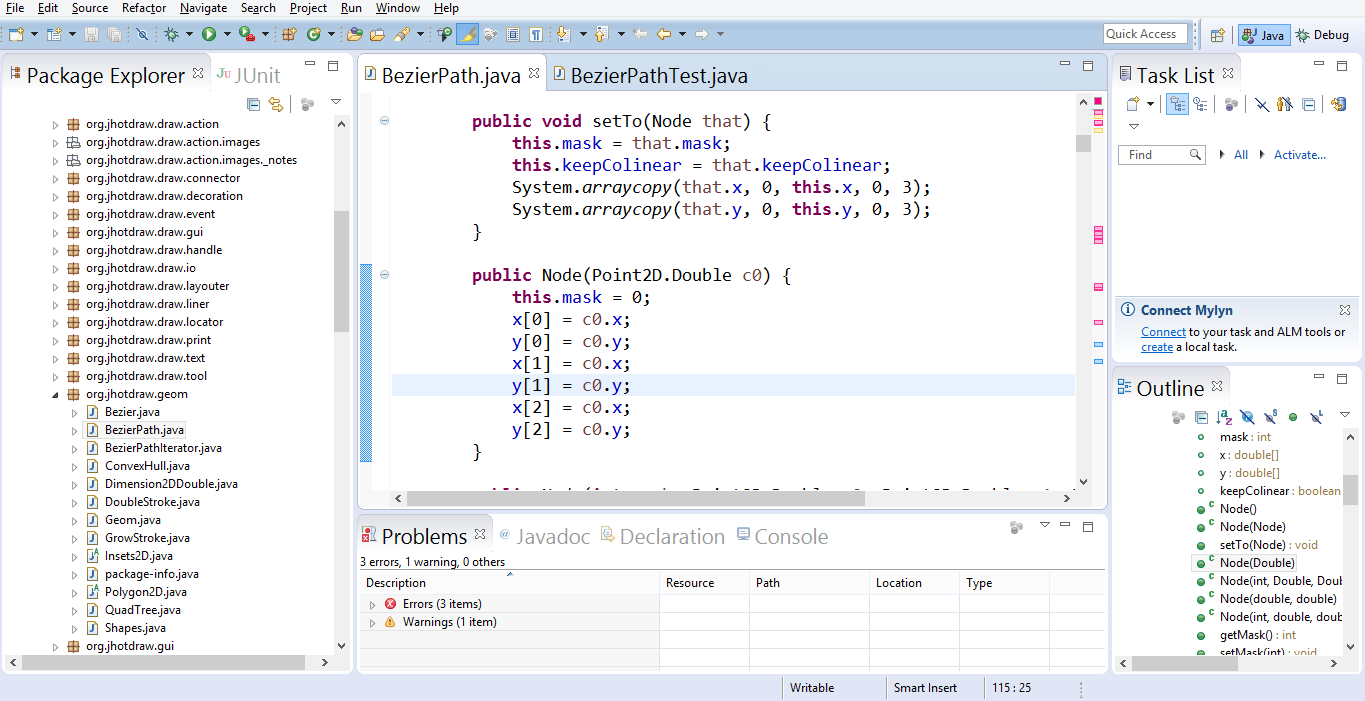
\includegraphics[scale=0.4]{screenshots/eclipseIntro3.png}
	\caption{Eclipse's user interface}
	\label{fig:Eclipse's user interface}
\end{figure}

In this section we describe current programming environments, namely Eclipse and
Pharo with respect to how unit test friendly they are. Special focus will be
placed on the features described in \autoref{cha:The Problem}. These features
are: viewing test and method side by side, search all tests for a specified
method and facilitating the creation of new tests. The two environments are
compared and possible places for improvement are discussed.

\section{Unit Testing in Eclipse}
\label{seg:Unit Testing in Eclipse}

We will start by taking a closer look at Eclipse since it is widely used and
many parallels to other programming environments (\eg Visual Studio) can be
made.

In \autoref{fig:Eclipse's user interface} you see a Java \brs{Say which project
this is and footnote a url to the repo or webpage}project opened in Eclipse
\ins{version bla bla}  with a package and two classes. The package and classes
can be seen on the left side in the ``Package Explorer'' pane.

\subsection{Methods and Tests Side by Side}

We start with a discussion on how Eclipse enables users to see \del{the} a
method and corresponding tests at the same time.

One option is to open both classes through the Package Explorer. The opened
classes will be shown in the middle of the screen and a new tab on top of the
code editor will appear.  In \autoref{fig:Eclipse's user interface} there are
two tabs ``\emph{BezierPath.java}''  and ``\emph{BezierPathTest.java}''.  The
``\emph{BezierPath.java}''  tab is currently selected and thus the content of
``\emph{BezierPath.java}'' is displayed in the code editor.  Unless you close
these tabs all the classes you opened will be quickly available through their
tabs.

A big advantage of this system is that users can create favorites by not closing
important tabs. Through this they can switch back and forth between methods and
tests. A slight drawback is that the user has to close unneeded tabs from time
to time to quicker find the currently important ones. In most cases the use of
these tabs will be smooth enough to allow the programmer to switch uninterrupted
between classes and their tests.

If for some reason this does not suffice then it is also possible to split the
code editor multiple times either horizontally or vertically like in
\autoref{fig:eclipseSplitscreen}. Since each code panel is smaller than the
original one this splitting can only be done a limited number of times. After
this the panels get too small to be useful.

As shown, Eclipse provides multiple ways to make the tested method easily
accessible during testing.

\begin{figure}[h]
	\centering
	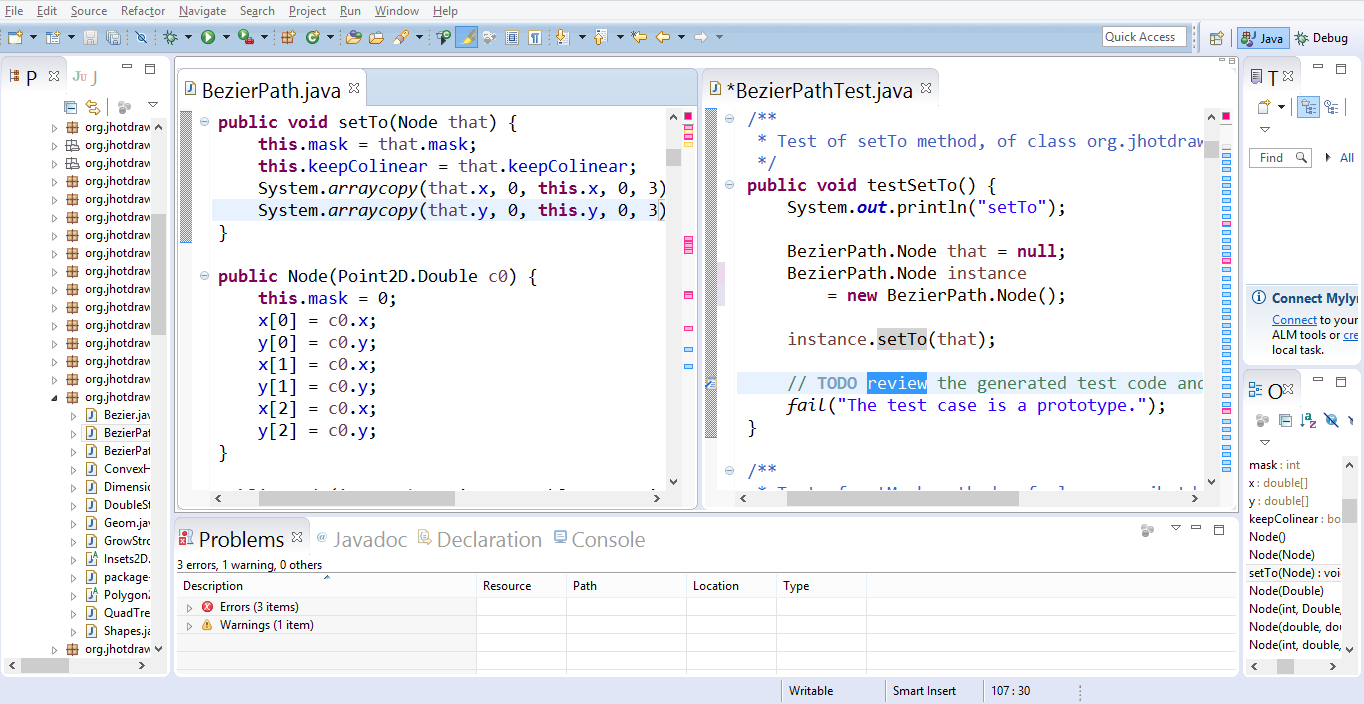
\includegraphics[scale=0.4]{screenshots/eclipseSplitscreen3.png}
	\caption{Split code panel}
	\label{fig:eclipseSplitscreen}
\end{figure}

\subsection{Test Search}

Another feature we discussed in the previous chapter was the ability to find all
tests of a certain method. Eclipse provides a good option to search for tests.
By selecting the "Search" from the top menu bar followed by "Referring Tests..."
it is possible to find all tests that reference the currently selected method.

Sadly this feature is very badly documented. The requirements for a test to
\del{to} be associated with a certain method seem to include that the test class
extends "TestCase" and that the test name starts with "test". \ins{The} "@Test"
annotations are ignored by this function. It seems like this test search does
not yet support JUnit 4 standards.

\subsection{Creating new Tests}

The next feature in Eclipse that we now discuss is how the creation of new tests
is facilitated. Eclipse provides an option for adding a new test class by right
clicking on the class that should be tested, selecting "New" from the list that
is shown and then clicking "JUnit Test Case".

In the newly open wizard a default name is already created and the selected
class is put into the "Class under test" field, \chg{see}{as shown in}
\autoref{fig:eclipseWizard1}. As default package the package of the class under
test is used but it can be changed. By clicking on the "Next" button it is
possible to select methods of the class under test and create test stubs for
every selected method, see \autoref{fig:eclipseWizard2}.

\begin{figure}[b!]
  \centering
  \begin{minipage}[b]{0.495\textwidth}
    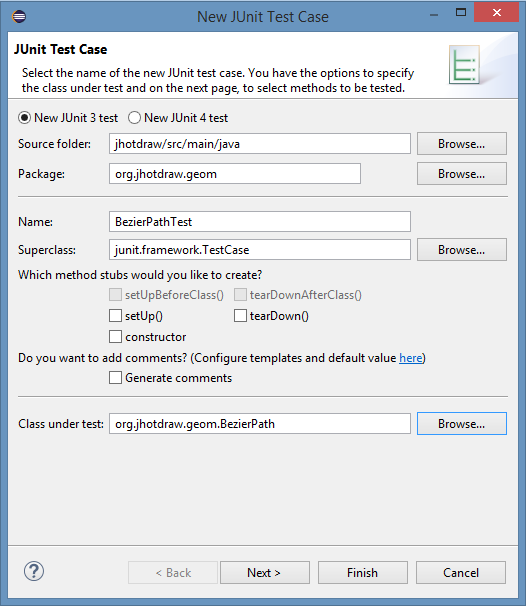
\includegraphics[width=\textwidth]{screenshots/eclipseWizard1_3.png}
    \caption{Test class wizard}
	\label{fig:eclipseWizard1}
  \end{minipage}
  \hfill
  \begin{minipage}[b]{0.495\textwidth}
    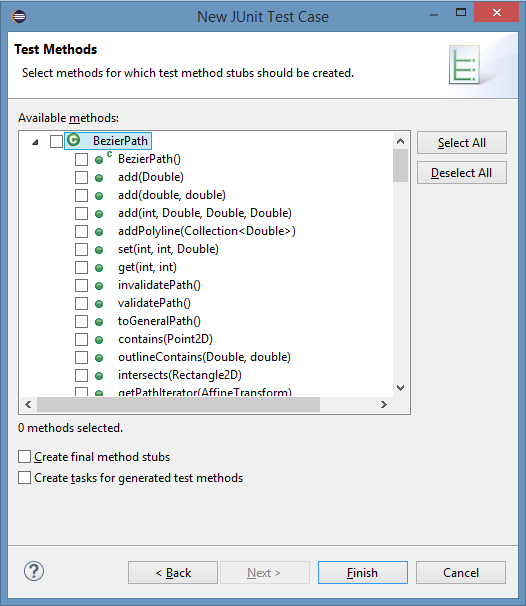
\includegraphics[width=\textwidth]{screenshots/eclipseWizard2_3.png}
    \caption{Select methods to test}
	\label{fig:eclipseWizard2}
  \end{minipage}
\end{figure}

On one hand, this wizard is very good for creating new test classes but on the
other hand Eclipse helps neither to add new test methods in an already existing
test class nor to create more than one test per method. During Test-Driven
Development its use is also limited, since it can only add tests to existing
methods.

\section{Unit Testing in Pharo}

Now let us take a look how the Pharo IDE and its system browser Nautilus support
unit testing and how they compare to Eclipse. In this context it seems worth
mentioning that the Pharo IDE is quite different from Eclipse in that the
placement of its visual elements is less rigid. The users are able to customize
the appearance of the environment very quickly and adapt it to their wishes. On
the other hand Pharo is less wide spread and not as well maintained in many ways
as Eclipse.

Like in \autoref{seg:Unit Testing in Eclipse} the discussed features are viewing
test and method side by side, searching all tests for a specified method and
facilitating the creation of new tests.

\subsection{Methods and Tests Side by Side}
\label{subsec:Nautilus side by side}

As with Eclipse the first functionality we will look at is the ability to view
tests and methods side by side. The Pharo IDE provides a very customizable
environment. It invites users to arrange all windows that are created in a way
that seems comfortable. It is possible to create multiple Nautilus windows and
arrange them so that one shows the method and the other the test for this
method. Through this a very similar effect to Eclipse's split code editor is
achieved.

The free placement of those Nautilus windows gives the user more freedom to
customize the environment but several visual elements will be duplicated which
reduces the available space on the screen to arrange these. An example for such
a duplicated element is the \ugh{file hierarchy}\brs{it's not a file hierarchy,
bur a list of packages and classes} that takes up the top half of each Nautilus
window like for example in \autoref{fig:Locking}.

A possibility that does not have this drawback is to lock a method or class and
then select others inside the same Nautilus window. It is possible to select
which of the locked elements is shown in the code panel by using the "All",
"Current" and number buttons shown at the bottom of \autoref{fig:Locking}.
Through these buttons the users can switch between seeing all locked methods and
classes at the same time or each individually. This is very similar to the tabs
of opened classes that Eclipse has. Although with many locked classes and
methods it is hard to remember which number belongs to what.

 \begin{figure}[h!]
	\centering
	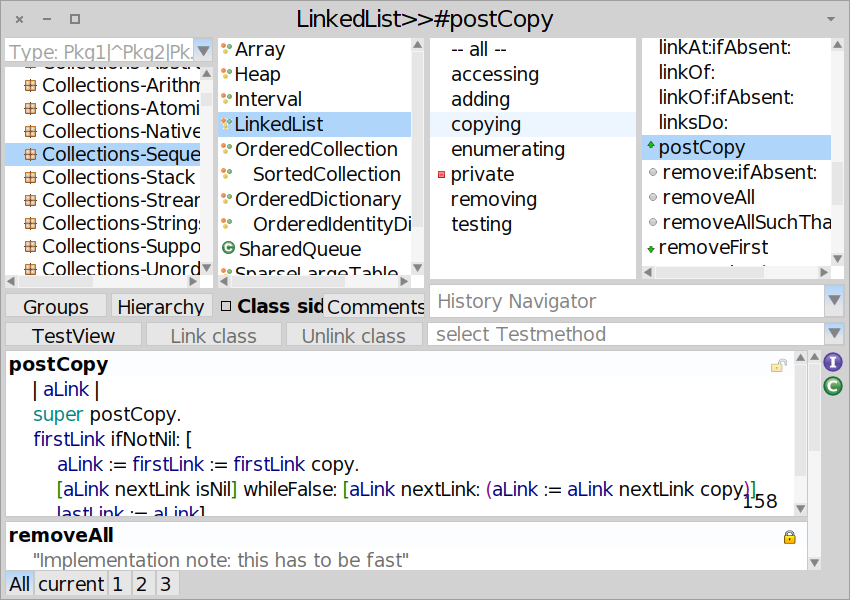
\includegraphics[scale=0.4]{screenshots/pharoLockedMethods2.png}
	\caption{Nautilus window with active locks}
	\label{fig:Locking}
\end{figure}

Apart from this Nautilus also has the History Navigator which allows fast access
to all recently viewed methods and classes. The History Navigator can be seen in
the middle right in \autoref{fig:Locking}. It can be used to switch between
method and test in a way that is comparable to Eclipse's tabs of recently opened
classes. The drawback here is that only a certain amount of those recently
accessed classes and methods is stored and if the user looks at different
methods and classes it is quickly necessary to reopen the previous tests and
methods to put them back in the History Navigator.

To conclude in the Pharo IDE are various things a user can do to view multiple
pieces of code at the same time. Compared to Eclipse there are more ways to see
things side by side or to switch between them but each of these ways has a
slight drawback.

\subsection{Test Search}
\label{subsec:Test Search}

The next functionality that will be discussed is how Pharo finds existing tests
for a specified method. Like Eclipse Nautilus has a test search implemented.
Like with Eclipse's test search only tests with \del{a} very specific
name\ins{s} are found. Additionally they have to be placed in classes with an
equally specific name.

Namely, test classes and test methods have to contain the full name of the class
or method under test. Additionally the name of the test class has to have the
suffix "Test" and the name of the test method has to have the prefix "test".
Also tests have no parameters and thus lack all colons in their name.  If
anything more is part of the test name then it will not be found by Nautilus's
test search. The test classes also have to inherit from
\chg{TestCase}{\emph{TestCase}}\brs{Emphasise the source code parts in text
somehow. Be consistent.} in order to be found by the test search. Examples of
tests corresponding to certain methods can be found in
\autoref{tab:correspondingMethods}.

\begin{table}[h!]
	\centering
	\begin{tabular}{| c | c || c | c |}
     	\hline
     	\emph{Class name} & \emph{Method name} &  \emph{Test class name} & \emph{Test name}\\ \hline
	AClassName & aMethodName & AClassNameTest & testAMethodName\\
	Nautilus & selectedClass & NautilusTest & testSelectedClass \\
	RxMatcher & matches: & RxMatcherTest & testMatches \\
	Stack & push: & StackTest &  testPush \\
	ProtoObject & ifNil:ifNotNil: & ProtoObjectTest & testIfNilIfNotNil \\
     	\hline
   	\end{tabular}
	\caption {Methods and corresponding \ugh{tests from Nautilus}\brs{these test
are not from Nautilus, they are the ones that can be found or generated by nautilus. Please
rephrase}}
	\label {tab:correspondingMethods}
\end{table}

Both the limitations on class names and method names are quite restrictive.
From a test class name the class under test can be quite reliably inferred. On
the other hand the method name and the corresponding test name for it are less
directly related\cite{Mars05a}. These restrictive name criteria also lead to the
problem that at most only one test per method will be found since others with a
slightly different name will not fulfill these naming criteria.

This test search function is not directly available to the developers. It is
used by Nautilus  in the file hierarchy to add a button to the left of each
method where a test has been found. This button can be pressed to execute the
test and show if this corresponding test was successful or not.

The test search is better in Eclipse since it is not only less restrictive with
its name-based criterion but also checks if the test calls the method under
test. Eclipse's test search is also able to find more than one test for a
method. On the other hand in Nautilus the test search is better integrated in
the environment. The additional button to execute a corresponding test
conveniently allows running the test without navigating to it.

\subsection{Creating new tests}

Right clicking on a method in Nautilus gives the "Generate test"  option.  The
new test will automatically be added to a certain test class in a specific
package (both of which will be created if needed). More precisely the test
package is named like the package under test with the suffix "-Tests". The test
class and method will be named like \autoref{tab:correspondingMethods} shows.
All the tests created through this will thus be found by Nautilus's test search
function.  "Generate test and jump" works very similar but also selects and
shows the newly created test so that the user can start implementing.

Using these predefined package and class names is faster since the user does not
need to enter them. Another advantage is that tests created in this manner
confirm to the naming standards imposed by Nautilus. Sadly this robs the user of
the ability to specify different package and class names. Also only one test per
method can be created in this manner. All additional tests for the same method
will simply overwrite the previous test since they will have exactly the same
name.

Eclipse's and Nautilus's way of adding new tests are very comparable. A case
could be made for both versions of this feature. Eclipse's version is more
customizable but only supports the user when creating a new test class while
Nautilus's version is faster and supports the user with each new test but is
less flexible. An easy way to create multiple tests for one method is not
provided by neither Nautilus nor Eclipse.

%%%%%%%%%%%%%%%%%%%%%%%%%%%%%%%%%%
%%%% The TestView Plugin %%%%%%%%%%%%%%%%%%%%%
%%%%%%%%%%%%%%%%%%%%%%%%%%%%%%%%%%
\chapter {The TestView Plugin}
	\label{cha:The TestView Plugin}

Having discussed some important features of a unit test friendly environment in
\autoref{cha:The Problem} and where their implementation is lacking in
\autoref{cha:Related Work} we will now present an attempt to address this
problem: the TestView Plugin.

Since the lack of unit test supporting features can not be corrected for all
environments at once we chose to extend Nautilus's functionality. The reasoning
behind this was that it is much easier to implement a plug-in for Nautilus than
for Eclipse. \ugh{Additionally the inability to view tests and methods side by side
in a single Nautilus window was perceived by us as the gravest of these issues
and that Eclipse already has a big community which provides many
plug-ins}\brs{how are these two connected? Side by side and eclipse community}.

In this chapter we will comment on how the TestView Plugin performs regarding
viewing test and method side by side, finding tests for certain methods and
creating new tests. Comparisons to Eclipse and the Pharo IDE will be drawn.

\section{Methods and Tests Side by Side}

As stated in \autoref{subsec:Nautilus side by side} one of the drawbacks
concerning unit testing with Nautilus is that it is hard to view tests and
methods at the same time. Whitebox testing becomes cumbersome through this.
Seeing both method and test together should be quick and convenient. It should
also not introduce too much redundant user interface elements that might clutter
up the environment.

Following this, the TestView Plugin allows splitting the code editor panel of a
Nautilus window vertically into two parts. The result of this can be seen in
\autoref{fig:Nautilus window with two code editors}. With this approach the need
to open two Nautilus windows is eliminated. The \ugh{file hierarchy} for example
will not be displayed a second time and less screen space is occupied.

\begin{figure}[h!]
	\centering
	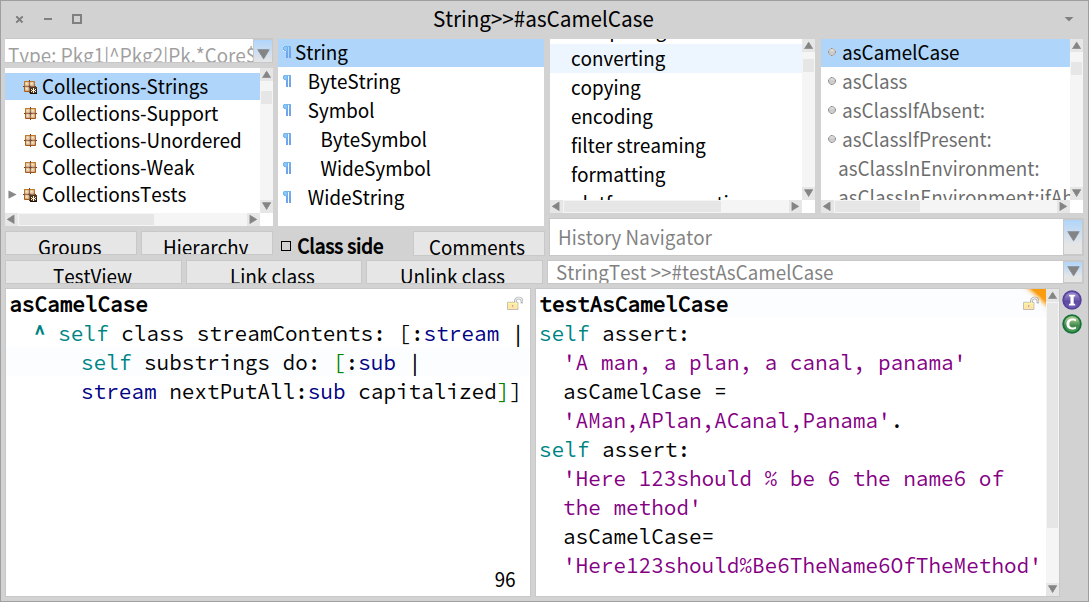
\includegraphics[scale=0.4]{screenshots/toggledOn2.png}
	\caption{Nautilus window with \ugh{two code editors}\brs{nope, it's the
nautilus editor with the TestView plugin installed right?}}
	\label{fig:Nautilus window with two code editors}
\end{figure}

It also becomes unnecessary to use Nautilus's locking feature or History
Navigator to be able to switch fast between methods and tests. Thus it also is
not required anymore to manage the locked or recently viewed classes and methods
in order to quickly navigate back and forth.

Unlike in Eclipse the user has no absolute control over this additional code
editor. Only methods of interest are shown there and the user does not have to
manage what should be displayed. This is possible due to the fact that some
assumptions can be made about what code the user wants to see if this code
editor is only used during unit testing. The left code editor will be displaying
the in the file hierarchy selected method and the right code editor will show
the corresponding tests.

Which test is currently shown can be changed through the drop list that can be
seen in \autoref{fig:Nautilus window with two code editors} just below of the
Nautilus History Navigator.

This approach combines the convenience of Eclipse's ability to show code side by
side with limited but more focused contend in the right code editor. This
results in an easy to use support for whitebox testing. Since it is not possible
to view multiple methods in one Nautilus window at the same time this is a
notable improvement.

\section{Test Search}

As a direct consequence of the heavily selected content of the second code
editor it became necessary to use a test search. Without this it would be
impossible to show a relevant selection. As discussed in \autoref{subsec:Test
Search} the test search that Nautilus provides is very restrictive and only
finds at most one test per method. In order to find better results the TestView
Plugin uses its own test search implementation.

\brs{use plug-in or plugin, just be consistent. Apply globally}

In the following subsections we will provide a detailed explanation how
corresponding tests for a certain method are found. The plugin uses a
hierarchical search with two stages. First the TestView Plugin searches all test
classes \chg{to}{of} the currently selected class and then inside of these test
classes all test methods \chg{to}{of}\brs{apply globally} the currently selected method.

This search is performed every time a different method is selected. This makes
it possible that the additional code panel introduced by the plugin always shows
a relevant selection.

\subsection{Corresponding Test Classes}
\label{subsec:CorrTestClasses}

A name-based search works quite well to find test classes corresponding to a
certain class\cite{Mars05a}. This is already used in the Nautilus test search
and a similar name based search is also part of the test search in the TestView
Plugin.

The name-based criterion requires the name of the class in question to contain
both the name of the selected class and an additional ``test''. This is why
``Contest'' is not considered to be a test class to a class that is also named
``Contest'' even though it contains ``test'' as well as the full name of the
class under test. The substring search is not case sensitive.

\brs{so, how is this different from what Nautilus does? I can see later that you
mention the ``inherits from TestCase'' situation, but please make that clear
first}

In \autoref{tab:TVTestClassNames} examples of which corresponding test classes
that the TestView Plugin finds are shown.

\begin{table}[h!]
	\centering
	\begin{tabular}{| c | c | c |}
     	\hline
     	\emph{Original Class Name} & \emph{Possible Class Names} &  \emph{Not Test Classes}\\ \hline
	String & StringTest, stringtest, TestString & String, Test, StrinTgEST \\
     	Contest & ContestTest, contesttest & Contest \\
     	\hline
   	\end{tabular}
	\caption {TestView name criterion for test classes}
	\label {tab:TVTestClassNames}
\end{table}

More precisely the name based search for test classes works as follows. First
all class names are gathered in a \textbf{class name collection}. In a
\textbf{substring collection} the name of the class under test and the string
``test'' is put. The substring collection is sorted so that the longest string
is first. Each element in the class name collection is now checked if it
contains the first string of the substring collection. If it does the first
occurrence of this substring is removed and it is checked if the remaining
string contains the second substring from the substring collection. Both
substring checks are not case sensitive. The naming criterion is fulfilled if
both substring checks are successful.\brs{wow that's confusing. Please rephrase
and give an example}

If a class  inherits from ``\emph{TestCase}'' in addition to fulfilling this
naming criterion the class is considered a corresponding test class\brs{so, you
do all this complicated stuff on ALL classes, and then filter the ones that are
actually tests? Please tell me you first filter the non test classes before
doing all the complicated stuff from the last paragraph}.

While a name-based test class search is quite precise a name-based test method
search is not. This lead us to first search for test classes and then in the
found test classes search for test methods. Since the test method search builds
on the results of the test class search it became important to make the test
class search works flawlessly\brs{bold claim, bring it down a bit \ie works as
good as possible}.

Our solution to this is to let the users customize the search results. If the
search for corresponding test classes is inadequate the developers can use the
``Link Class'' and ``Unlink Class'' buttons provided by the TestView Plugin to
add and remove test classes from the results.

Classes that have been unlinked will no longer be searched for test methods
while linked classes will be searched even if they do not inherit from
``\emph{TestCase}'' or fulfill the naming criterion. \ugh{If a class is linked and
unlinked multiple times only the latest input counts.}\brs{wat?}

The plugin keeps track of the linked and unlinked classes in two
\emph{Dictionaries}. When a class is linked or unlinked the currently selected
class is used as a key to store the specified class. Since the currently
selected class is used as a key each linking or unlinking of a class only counts
for the currently selected class. \ugh{It is possible that the user has to link or
unlink the same class multiple times for different classes.}\brs{again, wat? Why
do you insist on this multiple times thing without explaining why we care?}

\subsection{Corresponding Test Methods}

After some possible test classes have been identified using the criteria
described in \autoref{subsec:CorrTestClasses} the resulting classes will be
searched for corresponding test methods to the currently selected method.

Similar as the name criterion for test classes described in
\autoref{subsec:CorrTestClasses} the test methods have to contain the full name
of the selected method (without colons) as well as the string "test". Examples
can be found in \autoref{tab:testNameCrit}.

\begin{table}[h!]
	\centering
	\begin{tabular}{| c | c | c |}
     	\hline
     	\emph{Original method name} & \emph{Test names} & \emph{Not test names} \\ \hline
    	 addDays: & testAddDays & addDays, testAddDay \\
    	 asFloat & testFractionAsFloat, testFractionAsFloat2 & testFloatAsFraction \\
	print24:on: & testPrint24On, testPrint24OnWithPM & testPrint24withNanos \\
	 attest & attestTest, testAttest & attest \\
	\hline
   	\end{tabular}
	\caption {Test naming criterion}
	\label {tab:testNameCrit}
\end{table}

The substring search works like described in \autoref{subsec:CorrTestClasses}.
First a collection is created that contains all method names of all found
corresponding test classes. Then the substring collection is prepared. The only
difference here is that all colons are removed from the name of the selected
method before it is put in the substring collection. Like before the substring
collection is sorted according to length, both substring checks are made and
matches removed\brs{You are referring to an ugly section, so fix this one
accordingly once you fix the ugly one.}.

The second criterion besides the name criterion is that the test contains a
method invocation with the same selector as the selected method. If either of
those criteria is fulfilled the method is considered a test for the selected
method.

How many of those criteria are met is used to order the found tests in the
\ugh{droplist}\brs{drop down list or something, apply globally} that can be seen in
\autoref{fig:Nautilus window with two code editors} right below of the Nautilus
History Navigator. Specifically each found test method has an associated rating.
The rating is increased by one if the method uses the selected method and by two
if the naming criterion is fulfilled. Test methods with a higher rating will be
displayed first in the results.

This new search should yield better results than Nautilus' search since it
allows multiple test classes and methods to a particular method. It works very
similar to the test search provided by Eclipse and like Nautilus's search is
used directly by the IDE and does not have to be called manually.

\section{Creating new tests}

Another purpose of the TVPlugin is to make the creation of new tests as quick as
possible. This is done by providing the user with default names as much as
possible and making the creation of new test packages, classes and methods as
easy as possible.

Every time a developer starts to write a new unit test they have to determine to
which test class the new test belongs. We can split the creation of new tests
into two basic use cases: adding the new test in a new test class or adding the
new test in a test class where tests corresponding to the selected method
already exist.

\subsection{Adding a new Test Class}

First let us talk about what can be done to facilitate the creation of a new
test that does not yet have a fitting test class.  The easiest way to do this is
to let the users write the new test and later determine where this test will be
placed. With this the user is encouraged to immediately start writing a test as
soon as a method is created. The new test class option is activated by having
the topmost element ``new Test'' from the droplist of found tests\ins{as show in
figure bla}.

When the test method is saved the plugin will ask the user for the name of the
test class and in which package this class should be placed. Default values,
based on the class name and the package name of the method under test, are
provided. This might already be sufficient since test class names and test
package names can often be derived from the original class and package names
\cite{Mars05a}.

To create the default name for a new test package ``-Test'' is added to the name
of the package under test. Similarly the default test class name is derived from
the name of the class under test with the suffix ``Test''.

For example if the method under test is contained in a class called ``Queue''
within a package ``Collections'' then the proposed names for the test class and
the test package will be ``QueueTest'' and ``Collections-Tests''
\ins{respectively}. The new test class will also automatically subclass
TestCase.

These names and the inheritance from TestCase is also what Nautilus's test
search expects and thus this does not break existing conventions. Even though
default names are provided the user can still ignore them and specify different
ones.

\subsection{Adding a test to an existing Test Class}

The second use case is that a developer wants to add a test for a method that
already has tests. In this case the corresponding test classes should have
already been found by the plugin\brs{how? you don't really discuss how you know
it a method already has tests or not}. The users just have to select any test
that is in the test class where the new test should be added. No test package
has to be specified since only when a new test class is made the package might
also be a new one.

\ugh{One potential problem is how this choice between making new test classes and
test packages and using existing ones is communicated to the user. The users
have to make their intentions clear to the plugin by selecting a specific item
from the list of found tests.}\brs{no idea what this means}

When the user saves a test while having selected the first item in the
list\brs{what list?}\ins{,} the plugin will always ask the user to give names
for the test class and the test package. When the user has any other item
selected then the test is saved in the test class that was selected\brs{selected
where? Explain better and show figures of what you are talking about}. This might
create some confusion but on the other hand with only two clicks(open the list
and selecting target class) the user can specify where the new test should be
saved\brs{really needs to be rephrased}.

Now let us take a look at how this functionality compares to Eclipse and
Nautilus. Improvements compared to Eclipse are that the user can add a single
new test in an already existing test class. Eclipse has an advantage when
creating a new test class and filling it with multiple new tests. Eclipse
supports the user only at the start of writing a new test class while the
TVPlugin keeps supporting the user during the addition of any new test.

In Nautilus the user can extremely quickly create new tests in fixed test
packages and test classes but only one test per method can be created that way.
If the ``Generate test'' or the ``Generate test and jump'' option is pressed
multiple times then the previous test is overwritten. The TVPlugin helps the
programmers to add multiple tests to the same method.

%%%%%%%%%%%%%%%%%%%%%%%%%%%%%%%%%%
%%%% The Validation %%%%%%%%%%%%%%%%%%%%%
%%%%%%%%%%%%%%%%%%%%%%%%%%%%%%%%%%
\chapter {The Validation}
	\label{cha:The Validation}
%intro(aim, evaluation methods, )

To see if the TestView plugin fulfills our initial aim to encourage unit testing
we conducted a small scale controlled experiment coupled with a questionnaire.
Our most important research question was to see if the TestView plugin increases
test coverage by reminding the users to write tests. Other research questions
were if the plugin reduces the time, clicks and keystrokes necessary to
implement some simple classes and methods.

\section{The Setup}
%the participants
We evaluated the plugin with four people from the Software Composition Group of the University of Bern. The only requirements for the participants were that they know both the Pharo IDE and programming language.

%the evaluation
The evaluation was printed on multiple sheets in order to prevent later questions and tasks from influencing the participants. The evaluation started with two simple multiple choice questions surrounding test-driven development and unit testing. This was done to be able to group the participants according to how comfortable they were with testing. These questions were:

\begin{quote}
\begin{enumerate}
\item \label{itm:q1} Do you know what Test-driven Development is?


Yes		No
\item \label{itm:q2}How often do you write unit tests for your code?


Never		Rarely		Often		Always
\end{enumerate}
\end{quote}

The next part of the evaluation was the controlled experiment. For this we previously selected two problems. The participants were asked to write in the Pharo IDE a solution to these problems. One problem was the ``Even Fibonacci numbers''-problem\footnote{https://projecteuler.net/problem=2} and the other problem was the ``Sum Square Difference''-problem\footnote{https://projecteuler.net/problem=6}.

We paraphrased these problems taken from Project Euler to ensure that both tasks would require the same number of methods to complete:
\begin{quote}
\label{prob:fib}
Task1

Implement the ``Even Fibonacci numbers''-Problem.

(Hint the Fibonacci numbers are: 1,2,3,5,8,13,21,34,55,89,...)

a) Write a class with a method that generates all Fibonacci numbers below a certain number "collectFibBelow: aNumber".

b) Additionally the class should have a method to sum up all even numbers in a collection.

c) Write a method that combines a) and b) and sums up the even Fibonacci numbers below a certain number.
\end{quote}
\begin{quote}
\label{prob:sumDiff}
Task2

Implement the  ``Sum Square Difference''-Problem.

a) Write a method "sumSquaresOf: aCollection" that receives a collection of numbers, squares each number and sums up the squares.

b) Write a second method "squareSumOf: aCollection" that receives a collection of numbers, sums them up and returns the square of the sum.

c) Write a third method "sumSquareDiff: aCollection" that calculates the difference between "squareSumOf: aCollection" and "sumSquaresOf: aCollection".
\end{quote}

The participants were required to use a prepared laptop with two Pharo images. One image had the TV Plugin installed and the other did not. In each image one of the tasks had to be implemented. DFlow was used in both images to track the user interactions and the time.

To prevent the order of the images and the difficulty of the problems from influencing the evaluation we used counter balancing on both of these factors. This means that the first two people started both with the ``Even Fibonacci numbers''-Problem while the last two people ended with this problem. Every participant with an odd number started without the TVPlugin while those with an even number started the first task with it and then completed their second task without it.

The evaluation ended with an open question to gather opinions about the usefulness of the plugin:

\begin{quote}
\begin{enumerate}
\setcounter{enumi}{2}
\item \label{itm:q3}Did the TestView plug-in help in your opinion?
\end{enumerate}
\end{quote}

To measure if the plugin encourages the users to write test we used the test coverage percentage. We neither told the participants explicitly to write tests nor that the plugin was there. With this we wanted to see if simply by being there the plugin would remind users to write tests. Only if the participants decided to write tests we told them to use the plugin if they did not notice it.

To quantify the participants' performance  we took additional measurements. With these the participants that used the plugin and those that did not should be compared. This should give us an indication if the plugin facilitates testing or not.

\section{The Results}

As expected everyone answered question \ref{itm:q1} with yes. For question \ref{itm:q2} two participants each said to write unit tests rarely or often respectively.

The results of the experiments can be seen in \autoref{tab:eval1} and \autoref{tab:eval2}. The results seem pretty unexpected which might be due to the small number of participants. All measurements were taken with DFlow. The tracked values are:

\begin{enumerate}
		\item time to complete the task in seconds
		\item number of pressed keyboard keys
		\item number of mouse clicks
		\item number of opened windows
		\item test coverage percentage
\end{enumerate}

\begin{table}[h]
	\centering
	\begin{tabular}{| c | c | c | c | c | c | c | c |}
     	\hline
     	Participant&Problem&First Task&Time&Keys pressed&Clicks&Windows&Coverage \\ \hline
    	1&	SumDiff	&No		&581		&540		&65	&12	&0\\
	2&	Fibonacci	&Yes		& 1945	&1550 	& 542	& 24	& 100\\
	3&	Fibonacci	&No		&1089		&810		&287	&17	&0\\
	4 &	SumDiff	&Yes		&516		&486		& 91	& 5	& 0\\  \hline
	Average:&		&		&1033		&847		&246 &15 	&25\\
	\hline
   	\end{tabular}
	\caption {Results with the TV Plugin}
	\label {tab:eval1}
\end{table}

\begin{table}[h]
	\centering
	\begin{tabular}{| c | c | c | c | c | c | c | c |}
     	\hline
     	Participant&Problem&First Task&Time&Keys pressed&Clicks&Windows&Coverage \\ \hline
    	1 &	Fibonacci	&Yes	&702	& 687		& 89	&13	& 0\\
	2&	SumDiff	&No	&919	&739		&170	&9	&100\\
	3 &	SumDiff	&Yes	&433	& 261		&107	&4	& 0\\
	4&	Fibonacci	&No	&1023	&1178		&108	&8	&0\\ \hline
	Average&		&	&769	&716		&119	&8.5 	&25\\
	\hline
   	\end{tabular}
	\caption {Results without the TV Plugin}
	\label {tab:eval2}
\end{table}

The averages of the experiments with the TV Plugin seem to be slightly worse than those without. This is very surprising since except person two nobody used or noticed the plugin. Most likely the small number of participants made the differences between them the decisive factor.

Most people with the exception of person two did not do unit testing or make use of the TestView plugin. The one person that used the plugin has a test coverage of 100\% with or without the plugin. Also Person two was faster, pressed less keyboard or mouse buttons and opened less windows without the plugin. This difference is most likely due to the varying difficult of the problems. Everybody seemed to have more difficulty with the \hyperref[prob:fib]{Fibonacci problem}.

Interesting was that while only one person wrote unit tests everyone was testing if parts of their code worked as expected in the Pharo Playground. Testing definitively is a necessity but sometimes developers seem to prefer to do it manually. By making unit testing easier a lot of those manual test could hopefully become unit tests. That everybody answered positive to question \ref{itm:q3} underlines the need for additional unit testing tools and an environment that properly supports unit testing.

The participants also gave general feedback to the plugin. The two most mentioned points were that the plugin should stand out more and that there should be a quick option to run all the found tests.

If making the plugin stand out more is really necessary is debatable since this was only wished by people who did not see the plugin. While this certainly would help users to discover the plugin, other users that already know about it could possibly be annoyed by it standing out to much.

A quick option to run all the found tests would certainly be a useful addition to the plugin. Luckily there are already the Nautilus TestRunner and Nautilus itself that provide similar functionality. So while this might be an option, enhancing the existing tools would keep the number of required tools low.


%%%%%%%%%%%%%%%%%%%%%%%%%%%%%%%%%%
%%%% Conclusion and Future Work %%%%%%%%%%%%%%%%%%%%%
%%%%%%%%%%%%%%%%%%%%%%%%%%%%%%%%%%
\chapter {Conclusion and Future Work}
	\label{cha:Conclusion and Future Work}
%TODO
%ideas: lack of large scale test suit support in TV(allan page beatiful testing), creating methods and classes from tests to better support tdd, better tdd support in general, unit testing cant be condensed to these core functionalities(e.g. test result collection and displaying is equaly as important),
In which we step back, have a critical look at the entire work, then conclude, and learn what lays beyond this thesis.

%%%%%%%%%%%%%%%%%%%%%%%%%%%%%%%%%%
%%%% Anleitung zu wissenschaftlichen Arbeiten %%%%%%%%%%%%%%%%%%%%%
%%%%%%%%%%%%%%%%%%%%%%%%%%%%%%%%%%
\chapter {Anleitung zu wissenschaftlichen Arbeiten}
	\label{cha:Anleitung zu wissenschaftlichen Arbeiten}
\section {User Guide}
	\label{sec:User Guide}
\subsection{What's the TestView Plugin?}
	\label{subsec:What's a TestView Plugin?}

Nautilus is the default system browser in the current Pharo version. \autoref{fig:NautilusWindow} shows how a Nautilus window normally looks like.
\begin{figure}[H]
	\centering
	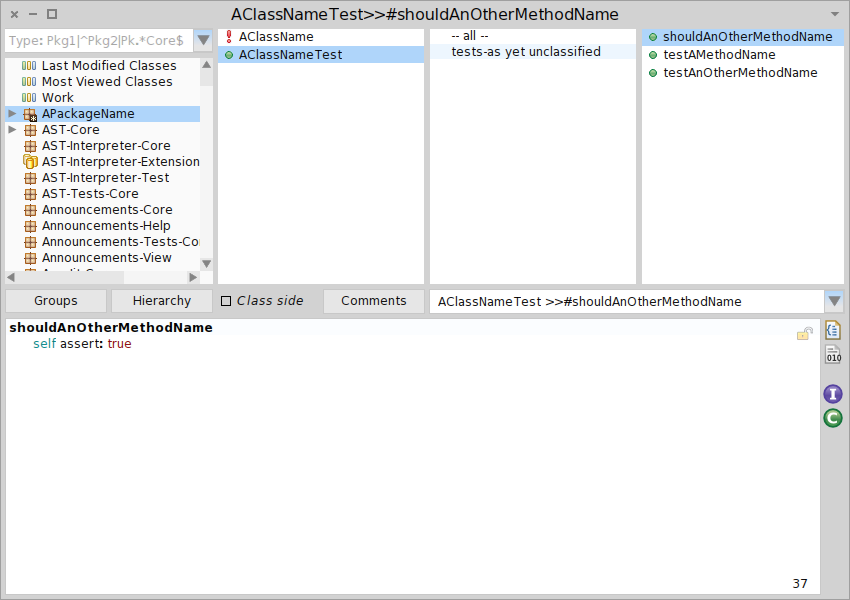
\includegraphics[scale=0.5]{screenshots/pharoClassHierarchy.png}
	\caption{A Nautilus Window}
	\label{fig:NautilusWindow}
\end{figure}
 The TestView Plugin (or TVPlugin) is a Nautilus plugin to facilitate unit testing. It provides quick ways to add new test methods and classes, find existing tests and view tests and methods at the same time in a single Nautilus window.


Let us take a look at the TVPlugin in \autoref{fig:TVPlugin overview} and discuss the features that it provides.
\begin{figure}[H]
	\centering
	\includegraphics[scale=0.5]{screenshots/tvPluginOverView_edited.png}
	\caption{Nautilus with the TVPlugin}
	\label{fig:TVPlugin overview}
\end{figure}
The \textbf{``TestView''} button toggles the additional code panel to the right of the original code panel on and off. All features described here require that the plugin is turned on.

The \textbf{selected method} is a central part of the plugin. All funtions the plugin provides are relative to what you have selected in the Nautilus window. Whenever you select a Method in the Nautilus class hierarchy the plugin will automatically search for corresponding tests.

In the \textbf{found tests droplist} every test corresponding to the selected method is shown. The first element in this list is special and will always be there independently from which method you have selected in the Nautilus window. Click this element to create a new test in a possibly new test class. How to do this is explained in detail in \autoref{subsec:Creating a new test inside a new test class}.
The remaining items in the list are all existing tests that are corresponding to the method you selected in the Nautilus window. By clicking on one of these the right code panel will display the selected test.

The \textbf{additional code panel} to the right of the original code panel will always show the test that has been selected in the found tests droplist. With this it becomes possible to look at the implemented method and at the tests for it inside of the same Nautilus window.

You can use the \textbf{``Link Class''} and \textbf{``Unlink Class'' buttons} if the found tests for the method you selected in the Nautilus window are incomplete or show methods that are not tests for what you selected. You can use both these buttons to influence the automated test search that gets performed whenever you select a different method in the Nautilus class hierarchy.

With the ``Link Class'' button you can specify a test class that is not found by the automated test search. The plugin will then redo the test search and include the newly linked class as a possible source for tests on every search to the class of the selected method.

With the ``Unlink Class'' button you can exclude classes from being searched for tests. Like with the ``Link Class'' button this exclusion will only count for the class of the method that you have currently selected in the Nautilus class hierarchy. Detailed instructions on how to use these functionalities are found in \autoref{subsec:Linking an existing test class} and \autoref{subsec:Unlinking an existing test class}.

\subsection{Installation and activation}
	\label{subsec:Installation and activation}
To install and activate the TVPlugin follow the steps listed bellow:

	\begin{enumerate}
		\item To download the necessary packages simply execute the following lines in a Pharo workspace
 \begin{code}
Gofer new
url: 'http://smalltalkhub.com/mc/DominicSina/TestView/main';
package: 'ConfigurationOfTestView';
load.
(Smalltalk at: #ConfigurationOfTestView) loadDevelopment.
NautilusPluginManager new openInWorld\end{code}
Once this is finished the Nautilus Plugins Manager will open.

		\item
		In the window shown in \autoref{fig:pluginManager} you click on "TVPlugin" under "Available plugin classes" and then press on the "Add" button. Click "Ok" to confirm.

		\parbox{\linewidth}{\centering
        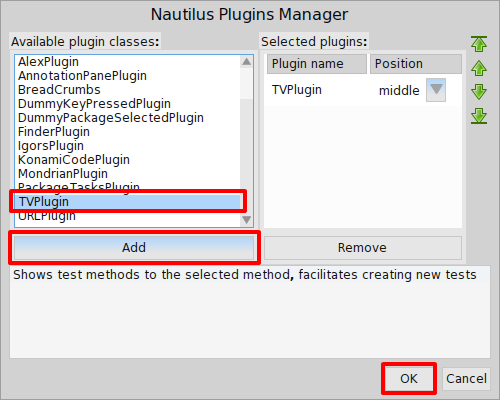
\includegraphics[scale=0.5]{screenshots/pluginManager_edited.png}
        \captionof{figure}{The Nautilus Plugin Manager}
	\label{fig:pluginManager}
    }

		\item
		When you open a Nautilus window from now it should look like in \autoref{fig:activeTVP}. To verify if the plugin is activated check if the highlighted row is displayed in the position that you selected. The plugin will be shown there until you remove it again using the Nautilus Plugins Manager.

		\parbox{\linewidth}{\centering
        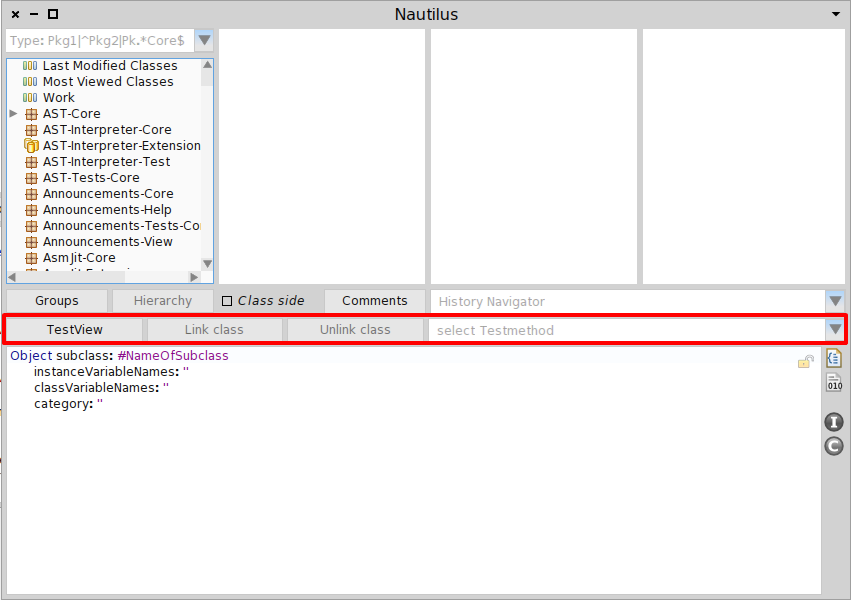
\includegraphics[scale=0.5]{screenshots/activatedPlugin_edited.png}
        \captionof{figure}{TestView Plugin once it is activated}
\label{fig:activeTVP}
    }

	\end{enumerate}

\subsection{Adding a new test inside a new test class}
	\label{subsec:Creating a new test inside a new test class}
So now that the plugin is set up after following the steps in \autoref{subsec:Installation and activation} let us add a new test for a method. In this example it is assumed that you have a method to test named ``doSomething'' inside of a class named ``MyClass'' and a package called ``MyPackage''.

\begin{enumerate}
\item Turn the TVPlugin on by clicking on the ``TestView'' button highlighted in \autoref{fig:toggleButton}. Once this is done a second code panel will appear besides the original code panel that shows a new test for your selected method.

		\parbox{\linewidth}{\centering
        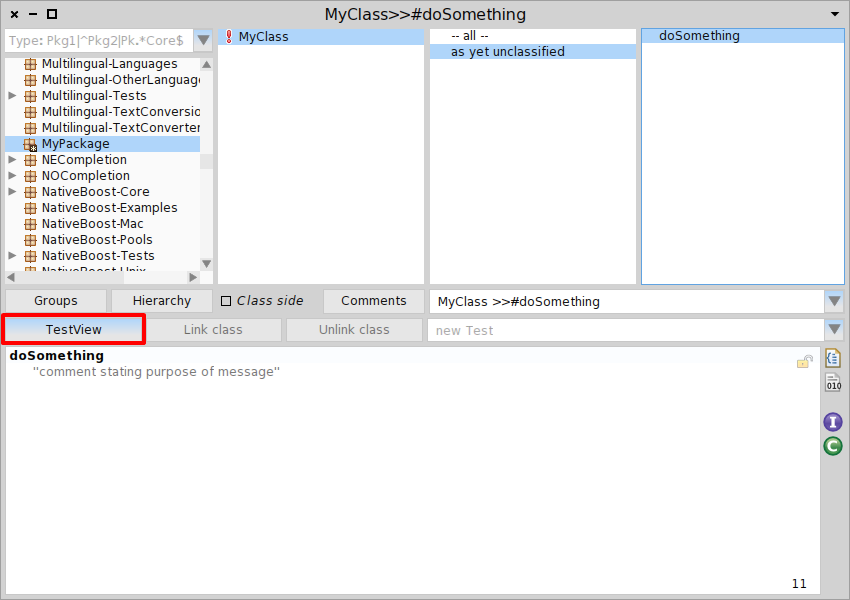
\includegraphics[scale=0.5]{screenshots/toggleButton_edited.png}
        \captionof{figure}{Toggle the TVPlugin on}
        \label{fig:toggleButton}
    }

\item Make sure that in the Nautilus window you have selected the method for which you want to add a test.

\item Now open the droplist showing all the tests that have been found for your method. Click on ``new Test'' as shown in \autoref{fig:dropListNewTest}. By doing this you signal to the plugin that you want to add a test in a new test class.

		\parbox{\linewidth}{\centering
        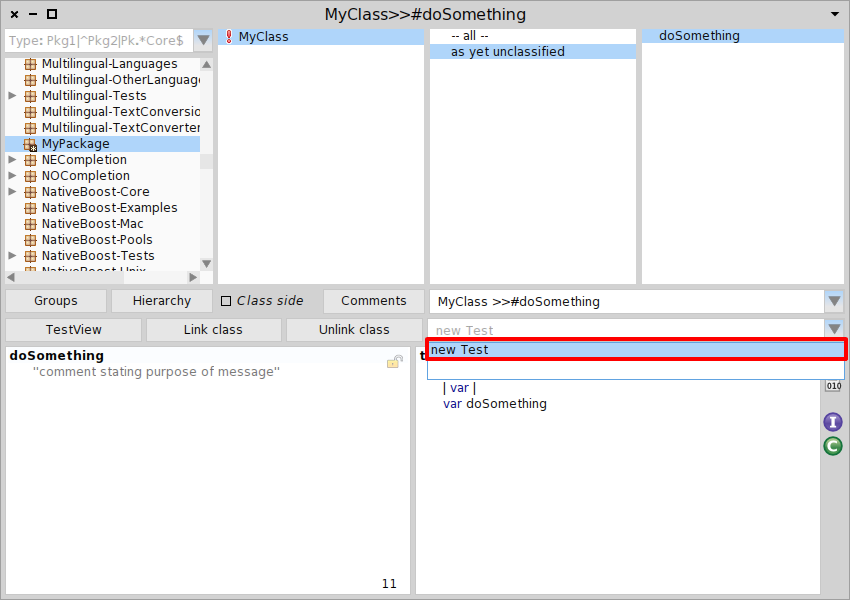
\includegraphics[scale=0.5]{screenshots/dropListNewTest_edited.png}
        \captionof{figure}{Signal that you want to save the test in a new test class}
\label{fig:dropListNewTest}
    }

\item Write your test in the right code panel. A template to start writing is already provided there by the TVPlugin.

\item Make sure the right code panel is still selected and accept your new test by pressing ctrl+s.

\item Since you previously selected ``new Test'' from the droplist the plugin is not sure in which test class this new test should be saved and will ask for clarification. As shown in \autoref{fig:newTestClassName} a default name will already be provided but you can write your own test class name. Click ``OK'' when you have entered a name.

		\parbox{\linewidth}{\centering
        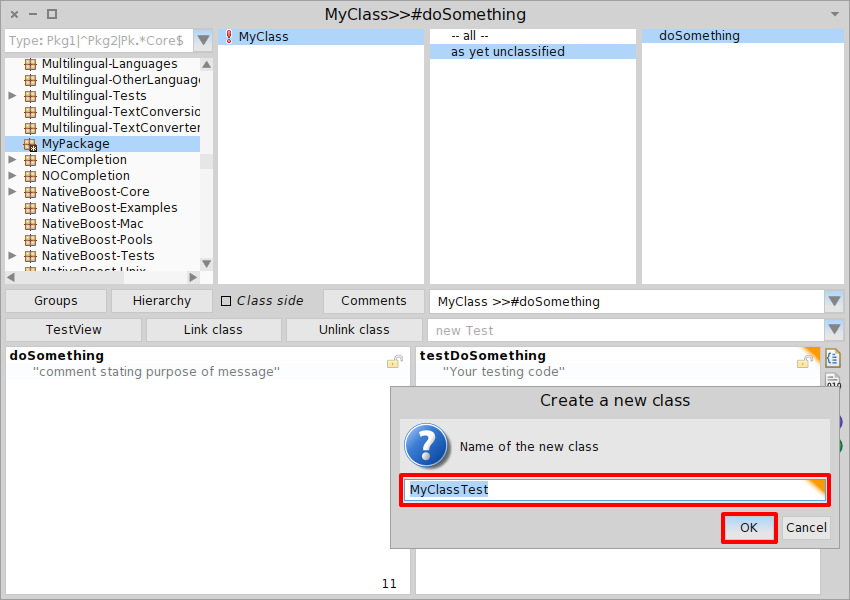
\includegraphics[scale=0.5]{screenshots/nameTestClass_edited.png}
        \captionof{figure}{Name the new test class}
\label{fig:newTestClassName}
	}

\item Now you need to name in which package this new test class will be added. Similarly as before a default name will be provided but you can enter your own. Click the ``OK'' button highlighted in \autoref{fig:newTestPackage} to confirm the package name. This test package will now be created if it did not exist previously.

  	\parbox{\linewidth}{\centering
        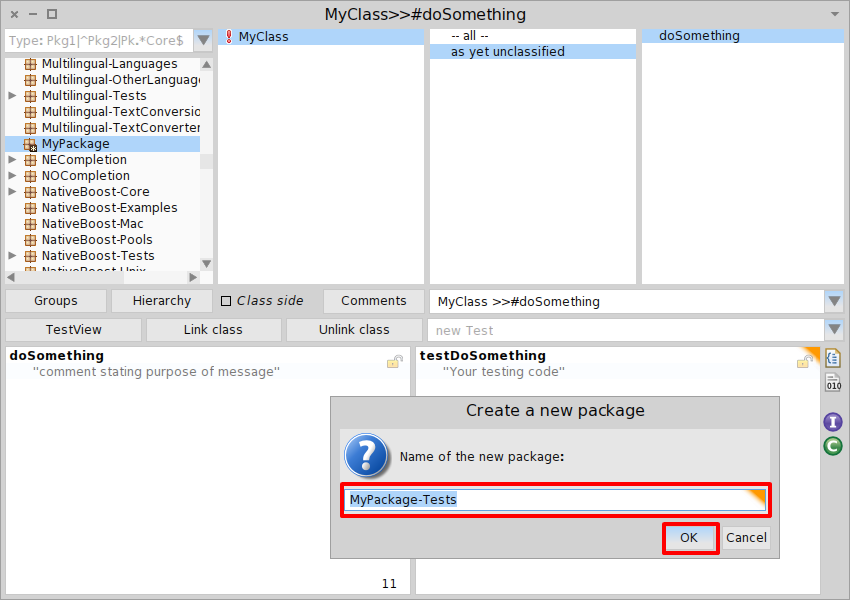
\includegraphics[scale=0.5]{screenshots/nameTestPackage_edited.png}
        \captionof{figure}{Name the new test Package}
\label{fig:newTestPackage}
	}

\item You will now see a pop-up similar to \autoref{fig:classConfirm} with a class definition according to what you entered in the previous steps. You can one last time change your mind and cancel the creation of the new class or enter new class and package names. Once you have finished checking and if necessary have made additional changes click on ``OK''. The new test will now be added to the newly created test class and test package.

	\parbox{\linewidth}{\centering
        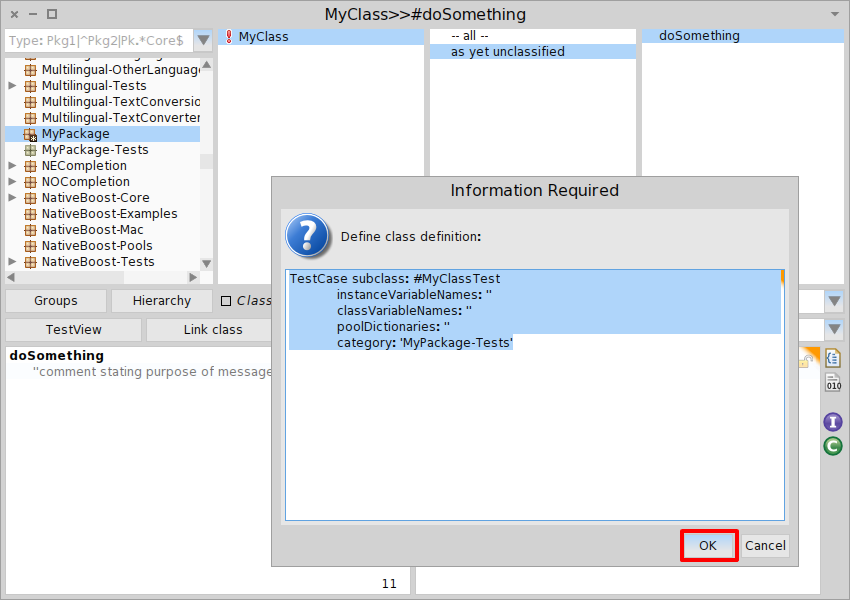
\includegraphics[scale=0.5]{screenshots/confirmNaming_edited.png}
        \captionof{figure}{Confirm the new test class}
\label{fig:classConfirm}
	}

\end{enumerate}

\subsection{Adding a new test to an existing test class}
	\label{subsec:Adding a new to an existing test class}
	In this section we will take a look at how to add a new test inside of an existing test class. It is assumed that the plugin is installed and activated. If not follow the steps outlined in \autoref{subsec:Installation and activation}.

\begin{enumerate}
	\item First make sure that the plugin is toggled on. If it is the Nautilus window has two code panels in the bottom. If it is not turn it on by clicking the ``TestView'' button. See \autoref{fig:toggleButton} if you can not find the button.

	\item Make sure that  in the Nautilus window you have selected the method for which you want to add a test.

	\item Now expand the droplist with the results and select any test that is contained in the class where you want your new test to be. In this example this will be ``MyClassTest'' so we select ``MyClassTest $>>$\#testDoSomething'' as can be seen in \autoref{fig:dropListExistingClass}.

	\parbox{\linewidth}{\centering
        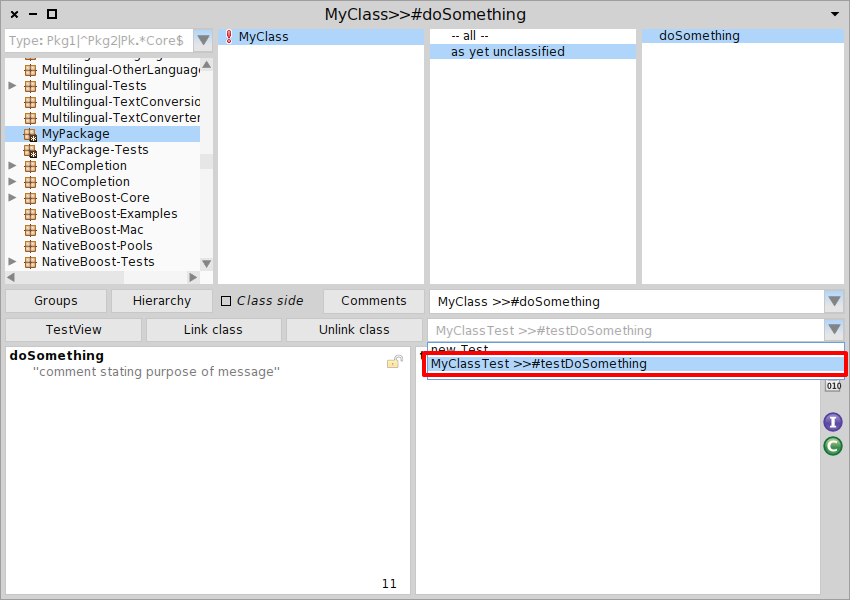
\includegraphics[scale=0.5]{screenshots/dropListExistingTestClass_edited.png}
        \captionof{figure}{Select any test in the desired test class}
\label{fig:dropListExistingClass}
	}

	\item The test you selected will now appear in the right code panel. Just write your test over it but make sure to give it a different name or else the test you selected will be overwritten.

	\item Make sure the right code panel is still selected and accept your new test by pressing ctrl+s.

	\item Now your new test will be added to the test class you selected previously. You can verify this by opening the found tests droplist again and checking if your new test is there as can be seen in \autoref{fig:newTestCheck}.

	\parbox{\linewidth}{\centering
        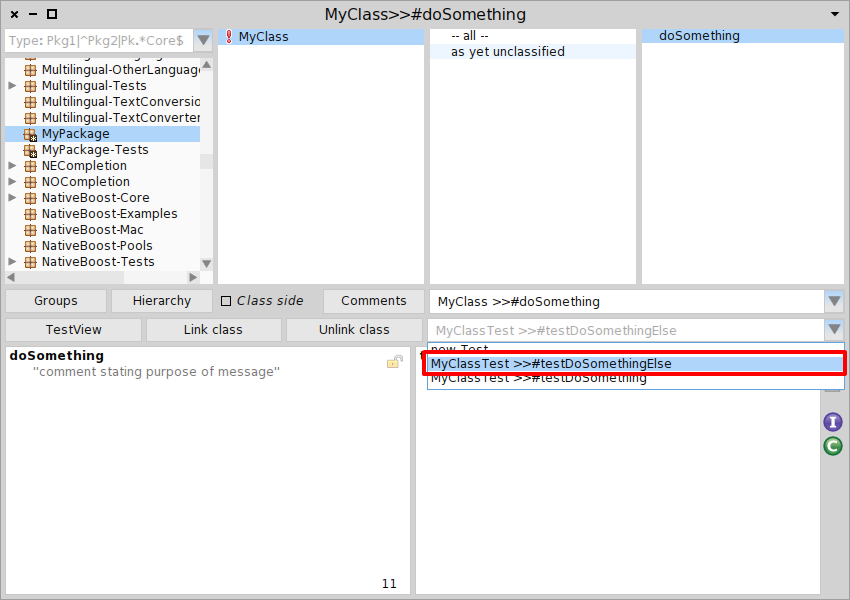
\includegraphics[scale=0.5]{screenshots/VerifyNewTestIsThere_edited.png}
        \captionof{figure}{Check if your new test is shown here}
\label{fig:newTestCheck}
	}
\end{enumerate}

\subsection{Linking an existing test class}
	\label{subsec:Linking an existing test class}
When the TVPlugin does not find tests that you have created then this might be because it does not recognize the your test class as a possible source for tests for the class of the method that you currently have selected in the Nautilus class hierarchy. Here you find a step by step list of how to add your test class to the considered test classes.

\begin{enumerate}
	\item First in the Nautilus class hierarchy select the method that is missing tests in the found tests droplist.

	\item Click the ``Link class'' button highlighted in \autoref{fig:linkClassButton}.

	\parbox{\linewidth}{\centering
        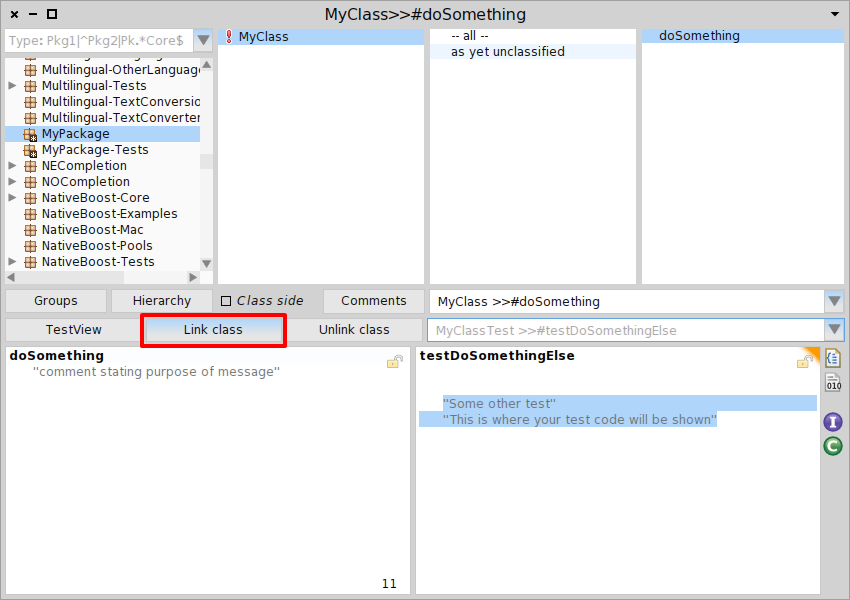
\includegraphics[scale=0.5]{screenshots/linkClassButton_edited.png}
        \captionof{figure}{The ``Link class'' button}
\label{fig:linkClassButton}
	}

	\item The TVPlugin will now ask which class you want to link as a test class to the class that is currently selected. Enter the name of the desired test class and click ``OK'' as shown in \autoref{fig:linkClassName}.

	\parbox{\linewidth}{\centering
        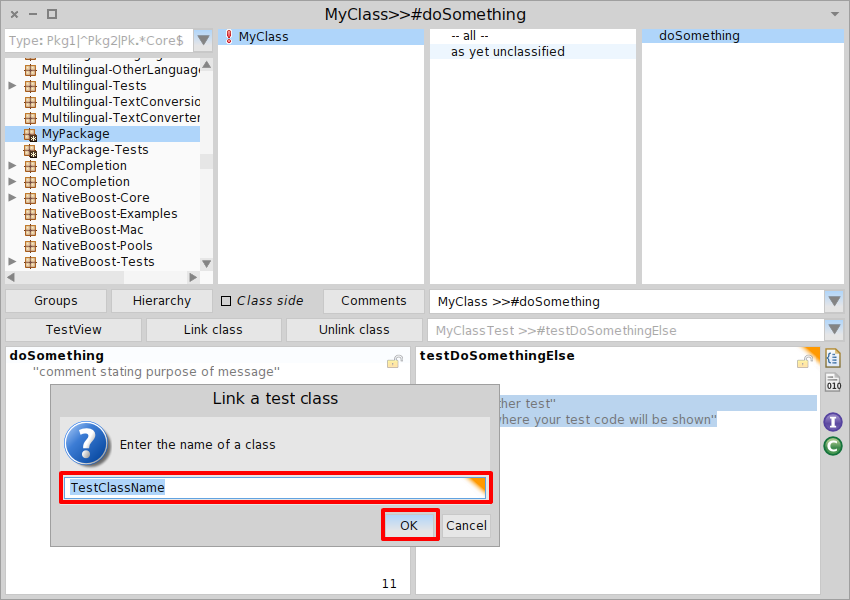
\includegraphics[scale=0.5]{screenshots/linkClassName_edited.png}
        \captionof{figure}{Pop-up asking for the test class name}
\label{fig:linkClassName}
	}

	\item The specified test class is now added to the test classes that will be considered when searching for tests for the currently selected class. You can verify if it now works by opening the found tests dropview.

\end{enumerate}

\subsection{Unlinking an existing test class}
	\label{subsec:Unlinking an existing test class}
In case the TVPlugin shows you tests from a test class that you do not recognize as a test class for the currently selected class you can remove this class from consideration by using the ``Unlink class'' button.

\begin{enumerate}
	\item First in the Nautilus class hierarchy select the method that does show too many tests in the found tests droplist.

	\item Click the ``Unlink class' ' button highlighted in \autoref{fig:unlinkClassName}.

	\parbox{\linewidth}{\centering
        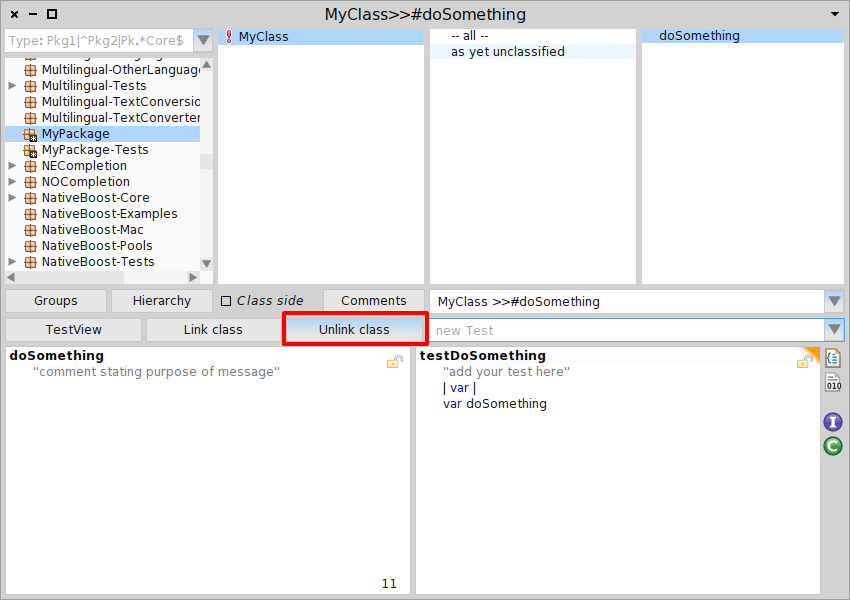
\includegraphics[scale=0.5]{screenshots/unlinkClassButton_edited.png}
        \captionof{figure}{The ``Unlink class'' button}
\label{fig:unlinkClassName}
	}

	\item The TVPlugin will now ask which class you want to unlink as a test class to the class that is currently selected. Enter the name of the desired test class and click ``OK'' as shown in \autoref{fig:unlinkClassName}.

	\parbox{\linewidth}{\centering
        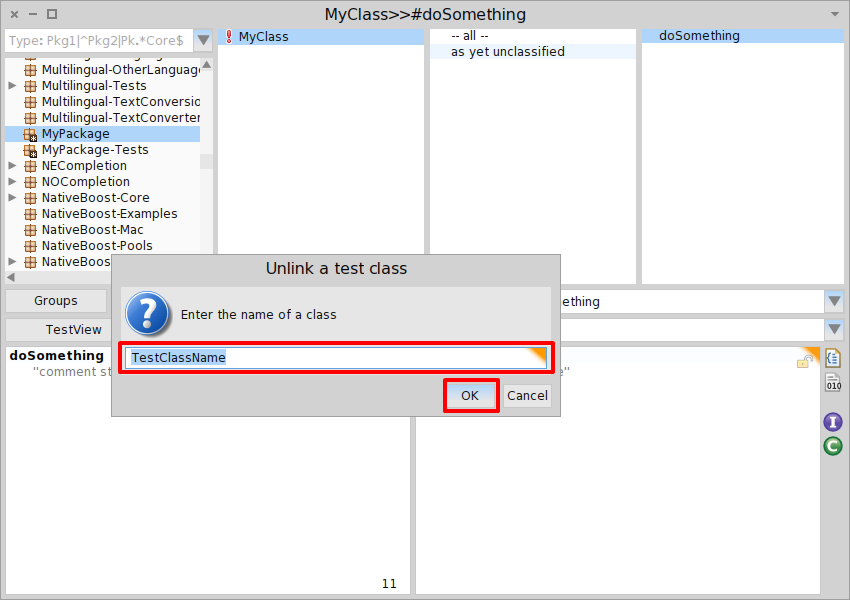
\includegraphics[scale=0.5]{screenshots/unlinkClassName_edited.png}
        \captionof{figure}{Pop-up asking for the test class name}
\label{fig:unlinkClassName}
	}

	\item The specified test class is now removed from consideration. All tests contained in this class will not be considered to be tests for the currently selected class. You can verify if this now works by opening the found tests droplist. No test contained in the unlinked class should be shown there.

\end{enumerate}

\subsection{Troubleshooting}
	\label{subsec:Troubleshooting}

	In this section possible problems with the TVPlugin are listed and possible solutions to them outlined.

	\subsubsection{Tests are not found by the TVPlugin}
		\label{subsubsec:Tests are not found by the TVPlugin}
In case all tests from one or multiple tests classes are missing in the found test droplist you can add those test classes manually by following \autoref{subsec:Linking an existing test class}. If you want to add individual tests from a test class where already some tests are found then continue with \autoref{subsubsec:Add and remove individual tests from the corresponding test list to the selected method}.

First make sure that your test classes are subclasses of ``TestCase''. If they are not the plugin will not consider them to be test classes. Simply go to the definition of your test classes and if necessary change the first line to ``[YourClassName] subclass: \#TestCase''. Check again if the tests from your test classes are found now by selecting the method for which some tests were not found.

If this does not help you can force the plugin to recognize your classes as test classes by linking the missing test classes to the currently selected class in the Nautilus class hierarchy. To do this follow the steps in \autoref{subsec:Linking an existing test class}. Recheck if your tests are found. If this does not work either then your tests themselves are written in a way that the TVPlugin does not recognize. You will have to change them so that they fulfill certain criteria. In this case also continue with \autoref{subsubsec:Add and remove individual tests from the corresponding test list to the selected method}.

\subsubsection{Tests that do not test the currently selected method are shown}
		\label{subsubsec:Tests that do not test the currently selected method are shown}
If the classes that contains these wrongly identified tests do not contain any tests for the currently selected class then you can simply unlink these classes. Follow the steps outlined in \autoref{subsec:Unlinking an existing test class}. All the tests from these classes should now be gone from the found tests droplist.

If you want to remove only some tests from the found tests droplist then continue with \autoref{subsubsec:Add and remove individual tests from the corresponding test list to the selected method}.

\subsubsection{Adding and removing specific found tests}
		\label{subsubsec:Add and remove individual tests from the corresponding test list to the selected method}
Both adding and removing an individual test from the tests that the TVPlugin finds are features that are directly supported. It is still possible to make these adjustments although likely not for all projects and not without changing your tests. The way the TVPlugin identifies individual tests as corresponding to the selected method has two components. The first one is solely based on the name of your test and the name of the method that it is supposed to test. The second one is if the test calls a method with the same name as the method that it supposedly tests.

The name based criterion is a check if your test contains the full name of your method under test with at least one additional time the substring "test". Examples of what is recognized as a test and what not based on this criterion are shown in \autoref{tab:name criterion examples}. This check is not case sensitive. ":" from methods names with parameters will be ignored when looking for a test.

\begin{table}[h!]
	\centering
	\begin{tabular}{| c | c | c |}
     	\hline
     	\emph{Original method name} & \emph{Test names} & \emph{Not test names} \\ \hline
    	 addDays: & testAddDays & addDays, testAddDay \\
    	 asFloat & testFractionAsFloat, testFractionAsFloat2 & testFloatAsFraction \\
	print24:on: & testPrint24On, testPrint24OnWithPM & testPrint24withNanos \\
	 attest & attestTest, testAttest & attest \\
	\hline
   	\end{tabular}
	\captionof{table}{Test naming criterion}
	\label{tab:name criterion examples}
\end{table}

The second criterion is if a method call is done inside of the possible test method to a method with the same name as the in the Nautilus class hierarchy selected method. This time the ":" are not removed from the check. If the supposed test method to a method named "do:on:" does call "doOn" then it will still not count as a test.

A test is recognized as such if either or both of these criteria are fulfilled. Conversely if neither is then the test is not considered a test for the selected method.
Adding a specific method to the tests found for a certain method can thus be done in two ways. Either make the name of the test contain the full name of the method in addition to "test" or call the method you want to test directly in the test. To remove a method from the found tests you have to make sure that the test name does not contain "test" and the full method name, and that inside of the test never a method with the same name as the supposed method under test is called.

\bibliography{scg,thesis}
	\bibliographystyle{plain}

\end{document}
